% !TEX program = pdflatex
% Laborbericht LEAS – Wechselrichter einphasig
% Bauen: Ctrl+Alt+B (LaTeX Workshop) oder  latexmk main.tex  (siehe README.md)
\documentclass[a4paper,11pt]{scrartcl}
% Pakete und Einstellungen – wird von main.tex eingebunden
\usepackage[T1]{fontenc}
\usepackage{lmodern}
\usepackage[ngerman]{babel}
\usepackage{csquotes}
\usepackage[a4paper,margin=2.5cm]{geometry}
\usepackage{microtype}
\usepackage{amsmath,amssymb}
\usepackage{siunitx}
\usepackage{booktabs}
\usepackage{graphicx}
\usepackage{caption}
\usepackage{subcaption}
\usepackage{tikz}
\usetikzlibrary{arrows.meta,calc,positioning}
% Farben der Zeigerdiagramme
\colorlet{cU}{blue!75!black}\colorlet{cI}{red!80!black}\colorlet{cD}{gray}
\colorlet{cP}{green!50!black}\colorlet{cQ}{orange!90!black}
\usepackage{pgfplots}
\pgfplotsset{compat=1.16}
% Offene Punkte als sichtbare Boxen. Vor der Abgabe:  [disable]  statt [textsize=footnotesize]
\usepackage[disable]{todonotes}
\usepackage[hidelinks]{hyperref}

\graphicspath{{img/}}
\captionsetup{font=small,labelfont=bf}

% Dezimalpunkt (Schweizer Schreibweise), Einheiten
\sisetup{output-decimal-marker={.},per-mode=symbol}
\DeclareSIUnit{\VAr}{var}

% Abkürzungen für Formelzeichen
\newcommand{\Udc}{U_{\mathrm{dc}}}
\newcommand{\UN}{U_{\mathrm{N}}}
\newcommand{\UWR}{U_{\mathrm{WR}}}
\newcommand{\uN}{u_{\mathrm{N}}}
\newcommand{\uWR}{u_{\mathrm{WR}}}
\newcommand{\iN}{i_{\mathrm{N}}}
\newcommand{\Th}{\vartheta}

% Gemeinsamer Stil für Diagramme
\pgfplotsset{
  rep/.style={width=0.92\linewidth,height=5.2cm,grid=major,
    tick label style={font=\small},label style={font=\small},
    legend style={font=\small},unbounded coords=jump}
}

\KOMAoptions{bibliography=totoc}

\begin{document}

% ---------------------------------------------------------------- Titelblatt
\begin{titlepage}
  \centering
  \vspace*{1.5cm}
  {\large Hochschule Luzern – Technik \& Architektur\par}
  {\large Modul LEAS\par}
  \vspace{2.5cm}
  {\Huge\bfseries Wechselrichter einphasig\par}
  \vspace{0.8cm}
  {\Large Laborbericht\par}
  \vspace{2.5cm}
  \begin{tabular}{@{}ll@{}}
    Autoren:      & Linus Brehm, Raphael Neidhart, Silas Jenzer  \\[2pt]
    Gruppe: & 5 \\[2pt]
    Dozent:         & Adrian Omlin \\[2pt]
    Messtage:       & 13.11.2026, 20.11.2026 und 27.11.2026 (Nachmessung) \\[2pt]
    Abgabe:         & 27.11.2026
  \end{tabular}
  \vfill
\end{titlepage}

\tableofcontents
\listoftodos[Offene Punkte]
\clearpage

% ---------------------------------------------------------------- Kapitel
% !TEX root = ../main.tex
\section{Einleitung}

\subsection{Ausgangslage}

Selbstgeführte Wechselrichter am Netz kommen in rückspeisefähigen Frequenzumrichtern (netzseitiger Teil), in Blindleistungskompensatoren und in Photovoltaik-Wechselrichtern vor. Die Versuchsanleitung (A.~Omlin, HSLU T\&A, Stand 08.11.2024) vergleicht drei Varianten für den netzseitigen Teil eines Frequenzumrichters (Tabelle~\ref{tab:varianten}).

\begin{table}[htbp]
  \centering
  \caption{Varianten des netzseitigen Teils eines Frequenzumrichters nach Versuchsanleitung.}
  \label{tab:varianten}
  \small
  \begin{tabular}{@{}p{3.6cm}p{3.6cm}p{3.2cm}p{4.2cm}@{}}
    \toprule
    Variante & Energiefluss & $\cos\varphi$ & Oberschwingungen \\
    \midrule
    Diodenbrücke & nur Netz $\to$ Last, kein Rückspeisen & -- & -- \\
    Umkehrgleichrichter (Thyristor) & beide Richtungen & vom Steuerwinkel abhängig, im Normalbetrieb deutlich $<1$ & durch die Schaltung weitgehend gegeben \\
    Selbstgeführter Wechselrichter (dieser Versuch) & beide Richtungen & frei einstellbar, z.\,B.\ $\cos\varphi=1$ & durch höhere Taktfrequenz und/oder geschickte Pulsmuster deutlich reduzierbar \\
    \bottomrule
  \end{tabular}
\end{table}

\subsection{Ziel des Versuchs}

Im Versuch werden das Funktionsprinzip sowie typische Strom- und Spannungsverläufe eines einphasigen, selbstgeführten Wechselrichters am Netz praktisch untersucht. Es soll gezeigt werden, wie sich Wirk- und Blindleistung einstellen lassen und wie sich Pulsmuster auf die Oberschwingungen auswirken. Die Messungen fanden am 13.11.2026 und am 20.11.2026 statt.

Gemäss Versuchsanleitung sollen die Studierenden

\begin{itemize}
  \item das theoretisch behandelte Verhalten des selbstgeführten einphasigen Stromrichters überprüfen,
  \item wissen, wie sich Wirkleistung und Blindleistung einstellen lassen,
  \item wissen, wie sich verschiedene Pulsmuster auf die Oberschwingungen auswirken,
  \item Spannungs- und Stromverläufe bei selbstgeführten Stromrichtern sicher interpretieren können.
\end{itemize}

\subsection{Aufbau des Berichts}

Der Bericht folgt dem Aufgabenraster der Versuchsanleitung. Kapitel~\ref{sec:aufbau} beschreibt Versuchsaufbau, Messpunkte und die verwendete Vorzeichenkonvention, Kapitel~\ref{sec:theorie} fasst die benötigte Theorie zusammen. Kapitel~\ref{sec:vorbereitung} behandelt die Vorbereitungsaufgabe (Aufgabe~5), Kapitel~\ref{sec:messungen} die Messaufgaben 6.1 bis 6.4. Abweichungen und Unstimmigkeiten werden in Kapitel~\ref{sec:diskussion} diskutiert, das Fazit steht in Kapitel~\ref{sec:fazit}.

% !TEX root = ../main.tex
\section{Versuchsaufbau und Messung}
\label{sec:aufbau}

\subsection{Leistungskreis}

Der Aufbau war fertig verkabelt (Abbildung~\ref{fig:blockschaltbild}). Die Asynchronmaschine (ASM) wird aus dem Netz~1 gespeist und treibt über die gemeinsame Welle die Gleichstrommaschine (GM). Der Anker der GM liegt am Zwischenkreis des einphasigen Wechselrichters (WR). Die Zwischenkreisspannung $\Udc$ wird über den Erregerstrom der GM (Klemmen F1/F2) eingestellt, die Drehzahl wird von der ASM praktisch konstant gehalten. Der Wechselrichterausgang ist über die Kopplungsinduktivität und einen Trenntransformator mit dem Netz~2 verbunden.

\begin{figure}[htbp]
  \centering
  \begin{tikzpicture}[
      blk/.style={draw,rectangle,minimum height=1.1cm,minimum width=1.4cm,align=center,font=\footnotesize},
      >={Stealth[length=2mm]},node distance=0.8cm]
    \node[blk] (n1) {Netz 1\\ $3\times\SI{400}{\volt}$};
    \node[blk,right=of n1] (asm) {ASM\\ \SI{5.5}{\kilo\watt}};
    \node[blk,right=of asm] (gm) {GM\\ \SI{6}{\kilo\watt}};
    \node[blk,right=of gm] (wr) {WR\\ IGBT-\\ Vollbrücke};
    \node[blk,right=of wr] (l) {$L$\\ \SI{70}{\milli\henry}};
    \node[blk,right=of l] (tr) {Trafo\\ $400/230$\,V};
    \node[blk,right=of tr] (n2) {Netz 2\\ \SI{230}{\volt}};
    \node[blk,below=0.8cm of gm] (err) {Erregung\\ F1/F2};
    \draw (n1) -- (asm);
    \draw[double distance=1.5pt] (asm) -- (gm);
    \draw (gm) -- (wr);
    \draw (wr) -- (l);
    \draw (l) -- (tr);
    \draw (tr) -- (n2);
    \draw[->] (err) -- (gm);
    \node[font=\scriptsize,above] at ($(gm.east)!0.5!(wr.west)$) {$\Udc$};
    \node[font=\scriptsize,above] at ($(wr.east)!0.5!(l.west)$) {$\uWR$};
    \node[font=\scriptsize,above] at ($(tr.east)!0.5!(n2.west)$) {$\uN$};
  \end{tikzpicture}
  \caption{Blockschaltbild des Versuchsaufbaus. Die Welle zwischen ASM und GM ist doppelt dargestellt; $\Udc$ wird über den Erregerstrom der GM eingestellt.}
  \label{fig:blockschaltbild}
\end{figure}

Der Wechselrichter ist ein synchronisierbarer Einphasenwechselrichter mit IGBT-Vollbrücke und antiparallelen Dioden, geteiltem Zwischenkreiskondensator (Mittelpunkt M.P.) und einem antiparallelen Koppelschalter auf der AC-Seite. Er hängt auf der \SI{230}{\volt}-Seite des Trenntransformators; bei einer Zwischenkreisspannung von $\Udc=\SI{259}{\volt}$ wurde eine Grundschwingung der Wechselrichterspannung von $U_1\approx\SI{233}{\volt}$ gemessen (Abschnitt~\ref{sec:messung611}).

Am Bedienfeld lassen sich der Winkel $\Th$ zwischen Wechselrichter- und Netzspannung (Tasten $\leftarrow$ $\rightarrow$), die Gleichspannung (Tasten $\uparrow$ $\downarrow$, wirkt auf die GM-Erregung), das Impulsmuster, die Synchronisation und das Koppeln bzw.\ Entkoppeln bedienen. Zur Verfügung stehen die geschlossene Rechteckschwingung (Grundfrequenztaktung), die Muster mit eliminierter 3.\ bis 5., 3.\ bis 9.\ und 3.\ bis 21.\ Oberschwingung sowie das Trägerverfahren (sinusbewertet) fein und grob.

\subsection{Geräte und Messpunkte}

Die Entkopplungsinduktivität hat \SI{70}{\milli\henry} (\SI{30}{\ampere}); bei \SI{50}{\hertz} ist $X=\omega L\approx\SI{22}{\ohm}$. Hinzu kommen ein Einphasentransformator $400/230$\,V (\SI{25}{\ampere}), eine Gleichstrommaschine (\SI{6}{\kilo\watt}, \SI{500}{\volt}) und eine Asynchronmaschine (\SI{5.5}{\kilo\watt}, $3\times\SI{400}{\volt}$). Gemessen wurde mit dem Voltech-Power-Analyzer PM\,3000 und seinem Spannungswahlschalter (Stellung «Netz»: $\uN$, Stellung «WR»: $\uWR$; der Strom ist immer $\iN$), dem Vierkanal-Oszilloskop Tektronix TPS2014 (isolierte Kanäle) mit Stromzange und Trennverstärkern, dem Multimeter Metra Hit 18S ($\Udc$) und einem optischen Drehzahlmesser. Tabelle~\ref{tab:messpunkte} nennt die Messpunkte.

\begin{table}[htbp]
  \centering
  \caption{Messpunkte der Grössen.}
  \label{tab:messpunkte}
  \small
  \begin{tabular}{@{}ll@{}}
    \toprule
    Grösse & Messort \\
    \midrule
    $\uN$ & Buchsen «Trenntransformator Sekundär» \\
    $\uWR$ & Buchsen direkt links der H-Brücke \\
    $\iN$ & Stromzange in der AC-Leitung \\
    $\Udc$ & Wechselrichter-Bedienfeld, Klemmen $+$ und $-$ \\
    $u_{\mathrm{Halbleiter}}$ & $+$ gegen obere $\uWR$-Buchse (oberer Schalter, linker Zweig) \\
    \bottomrule
  \end{tabular}
\end{table}

Für die Leistungsbetrachtung stand der Spannungswahlschalter des PM\,3000 auf «Netz». Nur für die Spannungsoberschwingungen von $\uWR$ wurde auf «WR» umgeschaltet; die Strom-Oberschwingungen wurden in Stellung «Netz» abgelesen.

\subsection{Vorzeichenkonvention}
\label{sec:vorzeichen}

Positive Wirkleistung $P>0$ bedeutet Leistungsfluss aus dem Netz~2 über Trenntransformator, Kopplungsinduktivität und Wechselrichter in die Gleichstrommaschine. Der Wechselrichter arbeitet dabei als Gleichrichter, die GM als Motor und die ASM als Generator, der in das Netz~1 speist. Bei $P<0$ wird Leistung in das Netz~2 zurückgespeist (Wechselrichterbetrieb, GM als Generator, ASM als Motor). Der Winkel $\Th$ ist der Nacheilwinkel der Grundschwingung von $\uWR$ gegenüber $\uN$; ein positives $\Th$ gehört zu $P>0$. Die Blindleistung $Q$ des PM\,3000 ist als $\sqrt{S^2-P^2}$ definiert und daher immer positiv; sie enthält die Verzerrungsblindleistung.

Die Winkelanzeige am Wechselrichter war gegenüber der in der Vorlesung gelernten Darstellung vorzeichenverkehrt. Dadurch wurden die Lastpunkte (Abschnitte~\ref{sec:messung621} und \ref{sec:messung64}) mit $P>0$ gefahren, also im Gleichrichterbetrieb mit der GM als Motor und der ASM als Generator, und nicht im Wechselrichterbetrieb. Nach Einschätzung der Gruppe ändert das an den Aussagen des Berichts nichts.

% !TEX root = ../main.tex
\section{Theorie}
\label{sec:theorie}

\subsection{Wirk- und Blindleistung}

Die Kopplungsinduktivität verbindet zwei Spannungsquellen: den Wechselrichter mit der Grundschwingung $\underline{U}_{\mathrm{WR1}}$ und das Netz mit $\underline{U}_{\mathrm N}$. Die Spannung $\underline{U}_{\mathrm N}$ wird als Bezugszeiger gewählt, $\underline{U}_{\mathrm{WR1}}$ eilt um den Winkel $\Th$ nach. Bei vernachlässigtem Widerstand fliesst der Strom
\begin{equation}
  \underline{I} = \frac{\underline{U}_{\mathrm N}-\underline{U}_{\mathrm{WR1}}}{\mathrm{j}X},
  \qquad \underline{U}_{\mathrm{WR1}} = U_{\mathrm{WR1}}\,\mathrm{e}^{-\mathrm{j}\Th},
  \qquad X=\omega L .
\end{equation}
Mit $\underline{S}=\underline{U}_{\mathrm N}\,\underline{I}^{*}=P+\mathrm{j}Q$ (Bezugssinn aus Sicht des Netzes, passend zur Konvention in Abschnitt~\ref{sec:vorzeichen}) folgt
\begin{equation}
  P=\frac{\UN\,U_{\mathrm{WR1}}\,\sin\Th}{X},
  \qquad
  Q=\frac{\UN\,\bigl(\UN-U_{\mathrm{WR1}}\cos\Th\bigr)}{X}.
  \label{eq:PQ}
\end{equation}
Die Wirkleistung wird also hauptsächlich über den Winkel $\Th$ eingestellt, die Blindleistung hauptsächlich über die Amplitude $U_{\mathrm{WR1}}$ und damit über $\Udc$. Das Verhalten entspricht dem Zeigerdiagramm einer Synchronmaschine am Netz, wobei $U_{\mathrm{WR1}}$ der Polradspannung entspricht. Die Blindleistung der Grundschwingung wird null für $U_{\mathrm{WR1}}\cos\Th=\UN$.

\subsection{Spannungs- und Stromoberschwingungen bei Grundfrequenztaktung}

Bei Grundfrequenztaktung ist $\uWR$ eine Rechteckspannung mit den Amplituden $\pm\Udc$. Die Fourier-Zerlegung enthält nur ungerade Ordnungen $n$:
\begin{equation}
  \uWR(t)=\frac{4\,\Udc}{\pi}\sum_{n=1,3,5,\dots}\frac{1}{n}\sin(n\omega t),
  \qquad
  U_{\mathrm{WR},n}=\frac{4}{\pi\sqrt2}\,\frac{\Udc}{n}\approx 0.9\,\frac{\Udc}{n}.
  \label{eq:rechteck}
\end{equation}
Die Netzspannung wird als sinusförmig angenommen, deshalb treiben nur die Oberschwingungen von $\uWR$ Oberschwingungsströme durch die Induktivität:
\begin{equation}
  I_n=\frac{U_{\mathrm{WR},n}}{n\,X}.
  \label{eq:In}
\end{equation}
Die Stromoberschwingungen fallen deshalb mit $1/n^2$ ab. Mit $L=\SI{70}{\milli\henry}$ ist $X=2\pi\cdot\SI{50}{\hertz}\cdot\SI{70}{\milli\henry}=\SI{22.0}{\ohm}$. Für $\Udc=\SI{259}{\volt}$ ergeben sich $U_{\mathrm{WR},1}=\SI{233.1}{\volt}$ und $U_{\mathrm{WR},3}=\SI{77.7}{\volt}$, $U_{\mathrm{WR},5}=\SI{46.6}{\volt}$, $U_{\mathrm{WR},7}=\SI{33.3}{\volt}$ sowie $I_3=\SI{1.18}{\ampere}$, $I_5=\SI{0.42}{\ampere}$, $I_7=\SI{0.22}{\ampere}$ (Vergleich mit der Messung in Tabelle~\ref{tab:611}).

Ist $U_{\mathrm{WR1}}=\UN$ und $\Th=0$, so verschwindet der Grundschwingungsstrom ($I_1\approx0$), und der Strom besteht nur aus Oberschwingungen.

\subsection{Leistungsgrössen mit Oberschwingungen}

Die Wirkleistung $P$ ist der Mittelwert von $u\cdot i$ über alle Frequenzen, $P_1=U_1 I_1\cos\varphi_1$ gehört zur Grundschwingung (Index 1). Da die Netzspannung nahezu sinusförmig ist, gilt $P\approx P_1$. Der PM\,3000 bildet $Q=\sqrt{S^2-P^2}$; diese Grösse enthält die Verzerrungsblindleistung und wird deshalb nie null. Erst die Grundschwingungsblindleistung $Q_1=\pm\sqrt{(U_1I_1)^2-P_1^2}$ kann durch null gehen. Der Phasenwinkel der 1.\ Harmonischen ist am PM\,3000 immer $\SI{0}{\degree}$, weil er auf die eigene Grundschwingung bezogen ist, und eignet sich deshalb nicht zur Bestimmung von $Q_1$. Bei festem $P$ liegt $Q_1=0$ dort, wo $I_1$ minimal wird. Der Leistungsfaktor $\lambda=P/S$ ist wegen der Oberschwingungen kleiner als $\cos\varphi_1$.

\subsection{Pulsmuster}

Bei Pulsmustern mit eliminierten Oberschwingungen werden Kerben an berechneten Winkeln gesetzt, die gezielt einzelne Ordnungen aus $\uWR$ entfernen. Beim Trägerverfahren folgt die Pulsbreite einem sinusförmigen Sollwert, die Oberschwingungen liegen dann um die Schaltfrequenz. Beide Verfahren verkleinern die Grundschwingung $U_{\mathrm{WR1}}$ pro Volt $\Udc$ gegenüber dem Rechteck; für denselben Lastpunkt ist deshalb eine höhere Zwischenkreisspannung nötig. Eine höhere Schaltfrequenz verschiebt die Oberschwingungen zu höheren Ordnungen, wo die Induktivität stärker dämpft, bedeutet aber mehr Schaltverluste und mehr EMV-Störungen (qualitative Aussage, nicht gemessen).

% !TEX root = ../main.tex
\section{Vorbereitung (Aufgabe 5)}
\label{sec:vorbereitung}

\subsection{Stromverlauf bei Grundfrequenztaktung}

Verlangt ist die Skizze des Stromverlaufs bei Grundfrequenztaktung unter der Annahme, dass die Grundschwingung der Wechselrichterspannung mit der Netzspannung übereinstimmt ($U_{\mathrm{WR1}}=\UN$, $\Th=0$). Die Spannung über der Induktivität ist dann $\uWR-\uN$, und es gilt $L\,\mathrm{d}i/\mathrm{d}t=\uWR-\uN$. Für die erste Halbperiode $0\le\omega t\le\pi$ mit $\uWR=+\Udc$ und $\uN=\hat U_{\mathrm N}\sin\omega t$ folgt durch Integration
\begin{equation}
  i(\omega t)=\frac{1}{X}\Bigl[\Udc\bigl(\omega t-\tfrac{\pi}{2}\bigr)+\hat U_{\mathrm N}\cos\omega t\Bigr],
  \qquad i(\omega t+\pi)=-i(\omega t).
  \label{eq:strom_vorb}
\end{equation}
Die Integrationskonstante ist so gewählt, dass der Strom mittelwertfrei ist. Mit $\hat U_{\mathrm N}=\sqrt2\cdot\SI{230}{\volt}=\SI{325.3}{\volt}$, $\Udc=\tfrac{\pi}{4}\hat U_{\mathrm N}=\SI{255.5}{\volt}$ und $X=\SI{22.0}{\ohm}$ ergibt sich der Verlauf in Abbildung~\ref{fig:strom_vorb} mit einem Scheitelwert von etwa \SI{3.5}{\ampere}. Der Strom besteht nur aus Oberschwingungen; seine Form entspricht dem Integral von «Rechteck minus Sinus».

\begin{figure}[htbp]
  \centering
  \begin{tikzpicture}
    \begin{axis}[rep,height=4.6cm,xlabel={$\omega t$ in \si{\degree}},ylabel={$u$ in V},
        xmin=0,xmax=360,xtick={0,90,...,360},ymin=-400,ymax=400,
        legend style={at={(0.5,1.04)},anchor=south,legend columns=2,font=\small}]
      \addplot[thick,domain=0:360,samples=721]{ifthenelse(x<180,255.46,-255.46)};
      \addlegendentry{$\uWR$ (Rechteck)}
      \addplot[thick,dashed,domain=0:360,samples=361]{325.27*sin(x)};
      \addlegendentry{$\uN$}
    \end{axis}
  \end{tikzpicture}

  \begin{tikzpicture}
    \begin{axis}[rep,height=4.6cm,xlabel={$\omega t$ in \si{\degree}},ylabel={$i$ in A},
        xmin=0,xmax=360,xtick={0,90,...,360},ymin=-5,ymax=5]
      \addplot[thick,domain=0:360,samples=721]{ifthenelse(x<180,(255.46*(x*pi/180-pi/2)+325.27*cos(x))/21.99,-(255.46*((x-180)*pi/180-pi/2)+325.27*cos(x-180))/21.99)};
    \end{axis}
  \end{tikzpicture}
  \caption{Berechnete Spannungen (oben) und Strom (unten) bei Grundfrequenztaktung mit $U_{\mathrm{WR1}}=\UN$ und $\Th=0$, nach \eqref{eq:strom_vorb}.}
  \label{fig:strom_vorb}
\end{figure}

\subsection{Beeinflussung von Wirk- und Blindleistung}

Abbildung~\ref{fig:zeiger} zeigt das Zeigerdiagramm mit dem Spannungsabfall $\Delta\underline U=\underline U_{\mathrm N}-\underline U_{\mathrm{WR1}}=\mathrm{j}X\underline I$ an der Kopplungsinduktivität; der Strom eilt $\Delta\underline U$ um \SI{90}{\degree} nach. Die Leistungen folgen aus \eqref{eq:PQ}:

\begin{itemize}
  \item Die \emph{Wirkleistung} wird über den Winkel $\Th$ zwischen $\underline U_{\mathrm{WR1}}$ und $\underline U_{\mathrm N}$ eingestellt, $P\propto\sin\Th$. Am Bedienfeld geschieht dies mit den Tasten für $\Th$.
  \item Die \emph{Blindleistung} wird über die Amplitude $U_{\mathrm{WR1}}$ eingestellt. Bei fester Pulsform ist $U_{\mathrm{WR1}}\propto\Udc$, am Versuch also über den Erregerstrom der GM. Ist $U_{\mathrm{WR1}}\cos\Th<\UN$, bezieht der Wechselrichter induktive Blindleistung aus dem Netz (untererregt); ist $U_{\mathrm{WR1}}\cos\Th>\UN$, liefert er induktive Blindleistung ans Netz (übererregt).
\end{itemize}

\begin{figure}[htbp]
  \centering
  \begin{tikzpicture}[>={Stealth[length=2.5mm]},scale=1.15]
    \coordinate (O) at (0,0);
    \coordinate (UN) at (4,0);
    \coordinate (UW) at (-25:3.6);
    \draw[->,thick] (O) -- (UN) node[right] {$\underline U_{\mathrm N}$};
    \draw[->,thick] (O) -- (UW) node[below right] {$\underline U_{\mathrm{WR1}}$};
    \draw[->,thick,dashed] (UW) -- (UN) node[midway,right,xshift=2pt] {$\Delta\underline U=\mathrm{j}X\underline I$};
    \draw[->,thick] (O) -- (1.5,-0.72) node[below right,xshift=-2pt] {$\underline I$};
    \draw (1.0,0) arc (0:-25:1.0);
    \node at (1.35,-0.2) {$\Th$};
  \end{tikzpicture}
  \caption{Zeigerdiagramm des einphasigen Wechselrichters am Netz bei $P>0$ (Bezug aus dem Netz); die Länge von $\underline I$ ist nicht massstäblich.}
  \label{fig:zeiger}
\end{figure}

% !TEX root = ../main.tex
\section{Messungen und Auswertung}
\label{sec:messungen}

Die Oszillogramme tragen die Zeitstempel des Oszilloskops (13.11.2026 für Aufgabe~6.1.1, 27.11.2026 für die Nachmessung von «3.\ und 5.\ eliminiert» und der Grundfrequenztaktung in Abbildung~\ref{fig:621}, 20.11.2026 für alle weiteren). Die Spuren sind an ihrer Form erkennbar (sinusförmige Netzspannung, pulsförmige Wechselrichterspannung, Netzstrom in Magenta); die Kanalfarben unterscheiden sich zwischen den Messtagen.

% ==========================================================================
\subsection{Aufgabe 6.1.1: Stromform bei Grundfrequenztaktung}
\label{sec:messung611}

Eingestellt wurden $\Th\approx\SI{0}{\degree}$ und $\Udc=\SI{259}{\volt}$. Der Grundschwingungsstrom liess sich nicht auf null bringen; sein Minimum betrug $I_1=\SI{0.827}{\ampere}$, was einer Spannungsdifferenz von rund \SI{18}{\volt} an $X=\SI{22}{\ohm}$ entspricht. Diese Differenz lässt sich mit dem Winkel-Offset aus Abschnitt~\ref{sec:messung612} erklären, sofern er an beiden Messtagen gleich war: Wird $P$ erst bei $\Th\approx\SI{4.7}{\degree}$ null, liegt bei angezeigtem $\Th\approx0$ effektiv ein Winkel von etwa \SI{4.7}{\degree} zwischen den Spannungen. Das ergibt $\Delta U\approx\SI{233}{\volt}\cdot\sin\SI{4.7}{\degree}\approx\SI{19}{\volt}$ und $I_1\approx\SI{0.87}{\ampere}$, was gut zum gemessenen Minimum passt (berechnet). Abbildung~\ref{fig:611} zeigt die Verläufe.

\begin{figure}[htbp]
  \centering
  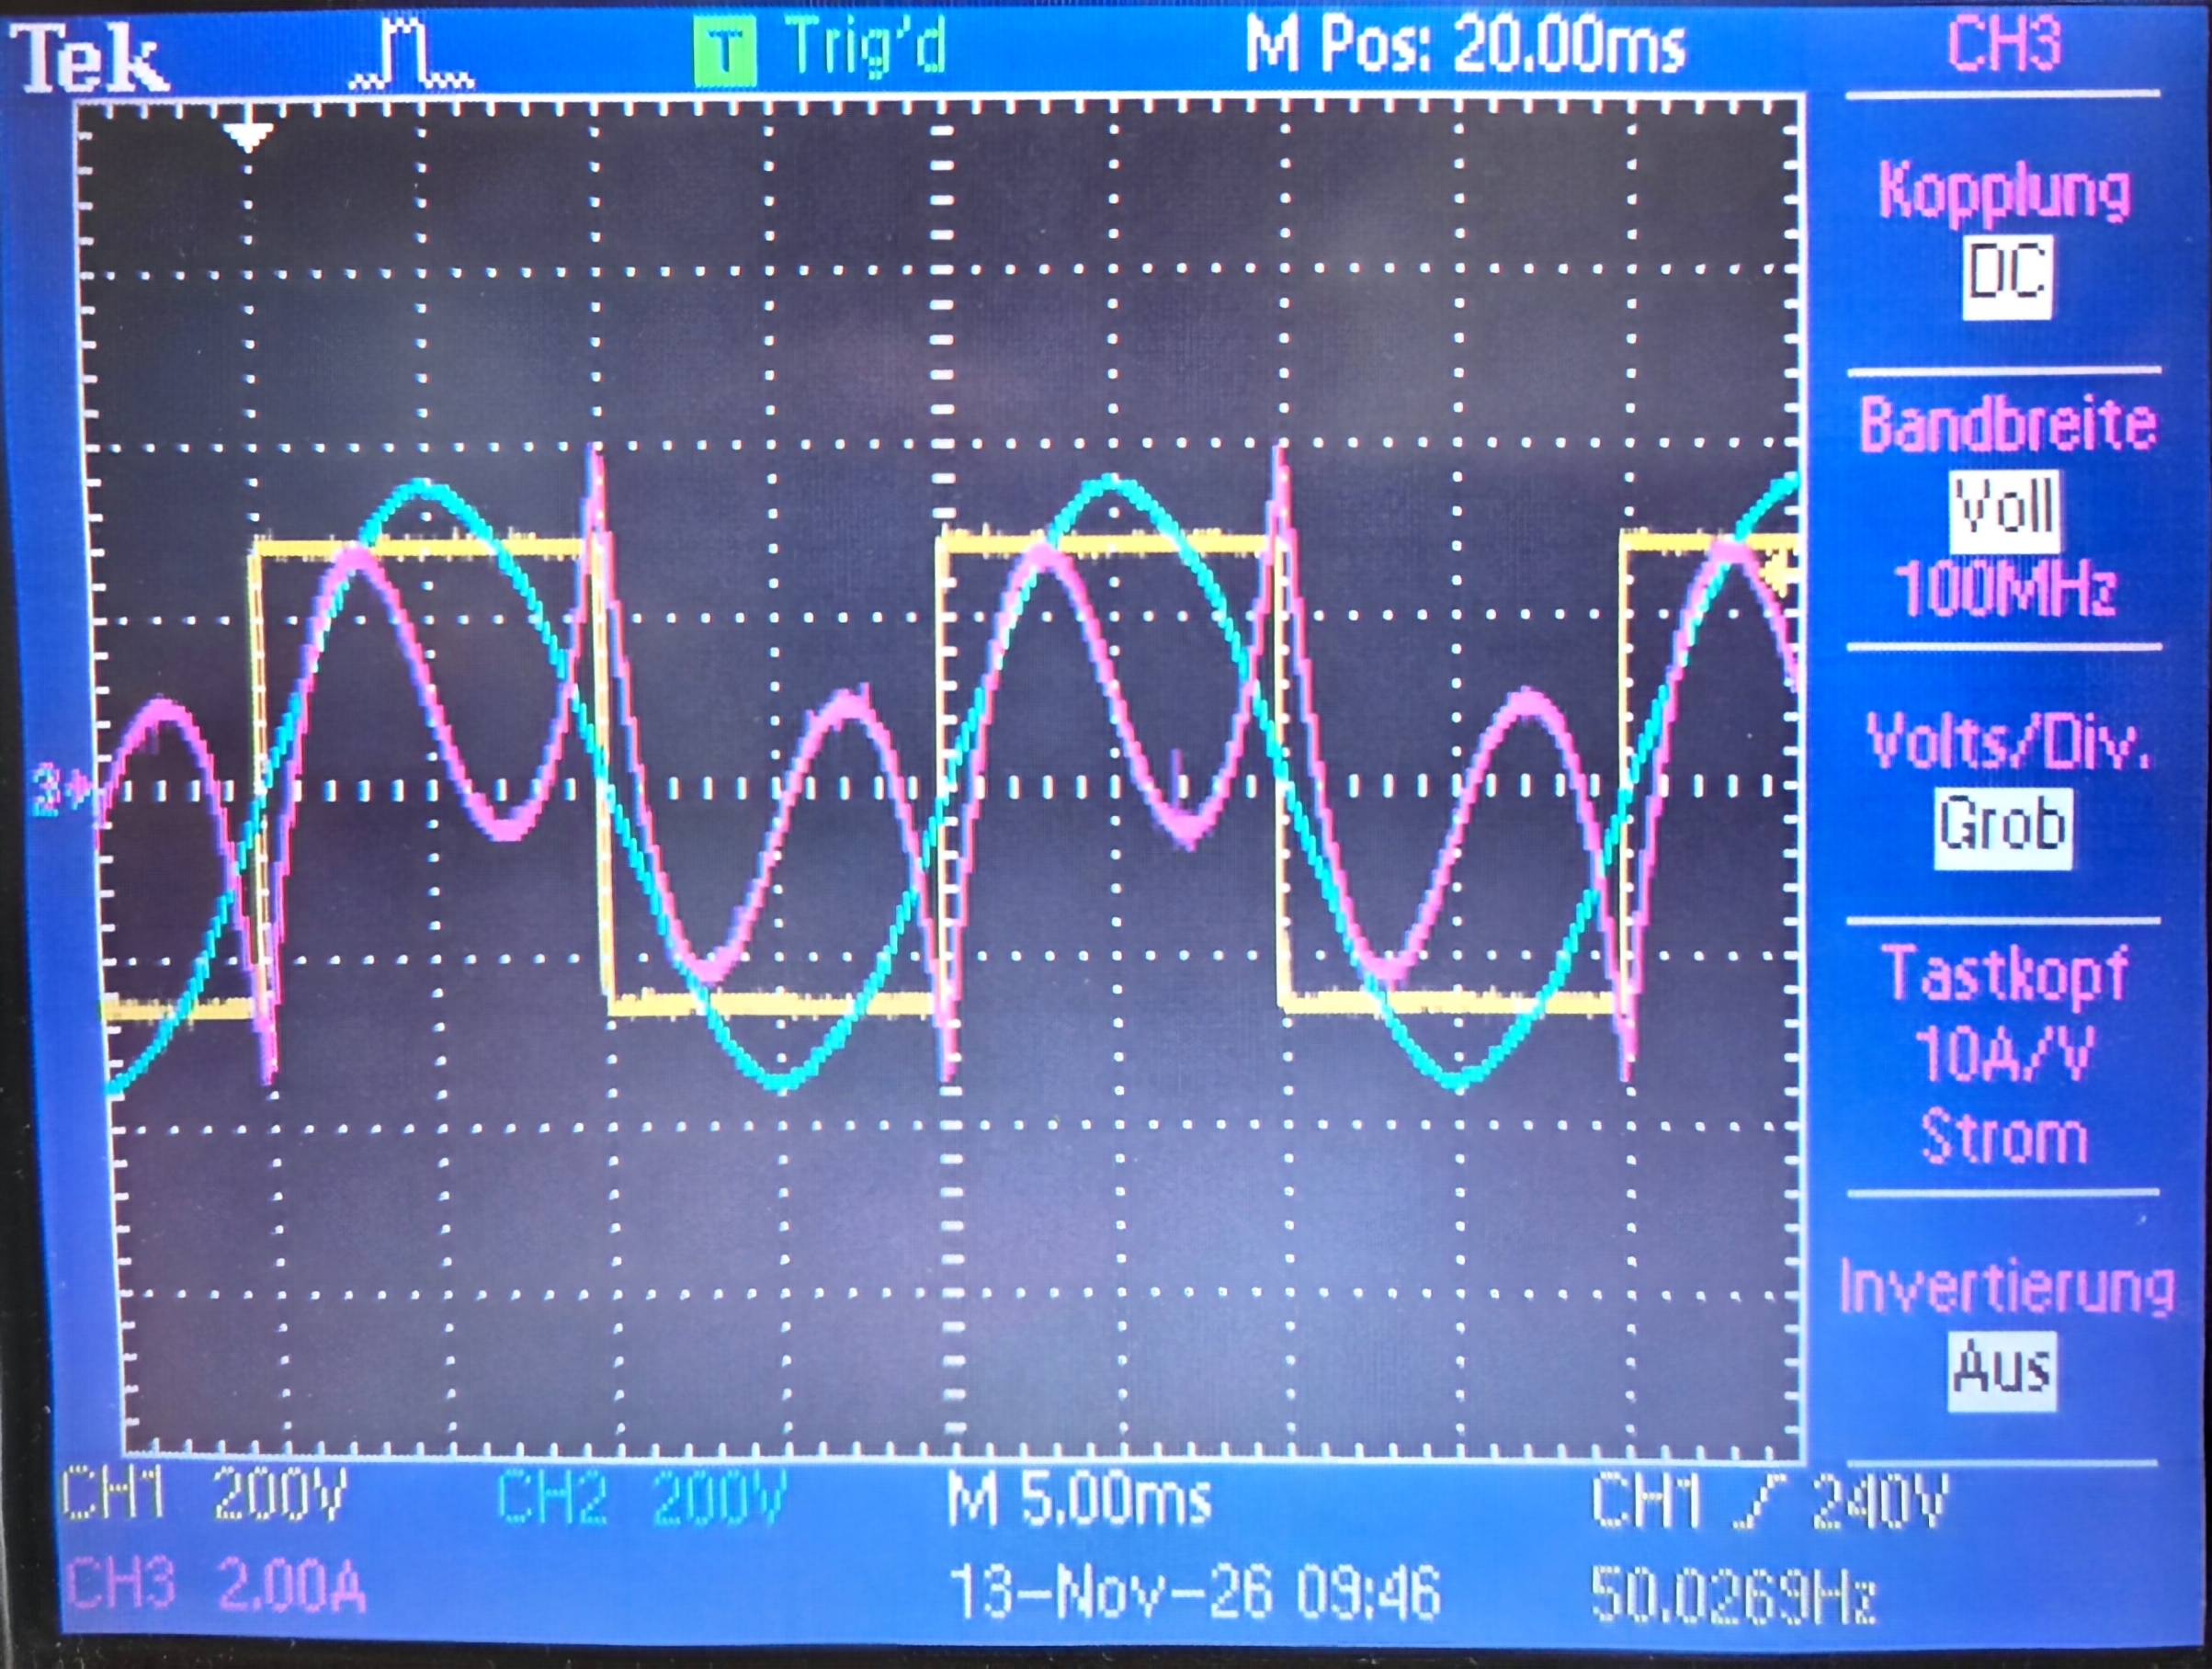
\includegraphics[width=0.62\linewidth]{Scan_20261113_101112.jpg}
  \caption{Aufgabe 6.1.1, Grundfrequenztaktung bei $\Udc=\SI{259}{\volt}$, $\Th\approx\SI{0}{\degree}$ (13.11.2026): rechteckförmige Wechselrichterspannung, sinusförmige Netzspannung und Netzstrom (Magenta). Skalen: \SI{200}{\volt}/div, \SI{2}{\ampere}/div, \SI{5}{\milli\second}/div.}
  \label{fig:611}
\end{figure}

Der Strom hat die erwartete Form aus Abschnitt~\ref{sec:vorbereitung}: Er besteht im Wesentlichen aus Oberschwingungen, und bei den Schaltflanken sind Stromspitzen zu erkennen. Tabelle~\ref{tab:611} vergleicht die am PM\,3000 abgelesenen Harmonischen mit der Theorie nach \eqref{eq:rechteck} und \eqref{eq:In}. Die Spannungsoberschwingungen wurden in Stellung «WR» gemessen, die Stromoberschwingungen in Stellung «Netz».

\begin{table}[htbp]
  \centering
  \caption{Oberschwingungen bei Grundfrequenztaktung, $\Udc=\SI{259}{\volt}$. $U_n$ in \% von $U_1$, $I_n$ in \% von $I_1=\SI{0.827}{\ampere}$. Theoretisch ist $I_1=0$ für $U_{\mathrm{WR1}}=\UN$ und $\Th=0$; der gemessene Restwert lässt sich mit dem Winkel-Offset erklären (siehe Text).}
  \label{tab:611}
  \begin{tabular}{@{}llrrrr@{}}
    \toprule
    & Ordnung $n$ & 1 & 3 & 5 & 7 \\
    \midrule
    $U_n$ & gemessen & \SI{233.3}{\volt} & \SI{33.42}{\percent} & \SI{19.87}{\percent} & \SI{14.32}{\percent} \\
    $U_n$ & Theorie ($0.9\,\Udc/n$) & \SI{233.1}{\volt} & \SI{33.3}{\percent} & \SI{20.0}{\percent} & \SI{14.3}{\percent} \\
    \midrule
    $I_n$ & gemessen & \SI{0.827}{\ampere} & \SI{145}{\percent} & \SI{50.5}{\percent} & \SI{28.4}{\percent} \\
    $I_n$ & Theorie & $\approx0$ (ideal) & \SI{142}{\percent} & \SI{51}{\percent} & \SI{26}{\percent} \\
    \bottomrule
  \end{tabular}
\end{table}

Spannung und Strom stimmen sehr gut mit der Theorie überein. Die Spannungsoberschwingungen fallen mit $1/n$, die Stromoberschwingungen mit $1/n^2$ ab. Die Abweichung der 7.\ Stromharmonischen (28.4 gegenüber 26\,\%) liegt vermutlich im Bereich der Ablesegenauigkeit.

% ==========================================================================
\subsection{Aufgabe 6.1.2: Einstellen von Wirk- und Blindleistung}
\label{sec:messung612}

Die Vorzeichenkonvention von $P$ und $\Th$ steht in Abschnitt~\ref{sec:vorzeichen}.

Abbildung~\ref{fig:zeiger612} zeigt qualitativ, wie sich die Zeiger und damit die Leistungen in den beiden Messreihen verändern. Wird nur $\Th$ verstellt (oben), dreht sich $\underline U_{\mathrm{WR1}}$ bei gleicher Länge um den Ursprung. Der Spannungsabfall $\Delta\underline U$ an der Induktivität steht dann nahezu senkrecht auf $\underline U_{\mathrm N}$, und der um \SI{90}{\degree} nacheilende Strom liegt fast in Phase ($\Th>0$, Bezug aus dem Netz) oder in Gegenphase ($\Th<0$, Rückspeisung) zur Netzspannung. Der grüne Wirkanteil wächst mit $\sin\Th$, der orange Blindanteil bleibt klein. Wird bei $\Th=0$ nur $\Udc$ und damit die Länge von $\underline U_{\mathrm{WR1}}$ verändert (unten), liegt $\Delta\underline U$ parallel zu $\underline U_{\mathrm N}$, und der Strom steht senkrecht dazu: Es entsteht nur ein Blindanteil. Bei $U_{\mathrm{WR1}}<\UN$ eilt der Strom nach, und der Wechselrichter bezieht induktive Blindleistung (untererregt); bei $U_{\mathrm{WR1}}>\UN$ eilt er vor (übererregt). Dieses Verhalten zeigen auch die Messreihen in den Abbildungen~\ref{fig:Ptheta} und \ref{fig:PUdc}.

\begin{figure}[htbp]
  \centering
  \begin{subfigure}[t]{0.32\linewidth}\centering
  \begin{tikzpicture}[>={Stealth[length=2mm]},scale=0.82,every node/.style={font=\scriptsize}]
    \path[use as bounding box] (-2.0,-1.9) rectangle (3.6,1.9);
    \draw[gray!40] (-1.9,0) -- (3.5,0);
    \draw[->,line width=1.4pt,cP] (0,0) -- (-1.423,0);
    \draw[->,line width=1.4pt,cQ] (-1.423,0) -- (-1.423,-0.251);
    \draw[->,thick,cI] (0,0) -- (-1.423,-0.251) node[above] {$\underline I$};
    \draw[->,thick] (0,0) -- (2.600,0) node[above right=-1pt] {$\underline U_{\mathrm N}$};
    \draw[->,thick,cU] (0,0.0) -- (2.443,0.889) node[above right=-1pt] {$\underline U_{\mathrm{WR1}}$};
    \draw[->,thick,dashed,cD] (2.443,0.889) -- (2.600,0);
    \draw[cU] (1.9,0) arc (0:20:1.9);
    \node[cU] at (2.167,0.382) {$\Th$};
    \node[align=center] at (0.8,-1.65) {\textcolor{cP}{$P<0$}, \textcolor{cQ}{$Q$ klein}};
  \end{tikzpicture}
  \caption{$\Th=\SI{-20}{\degree}$, $U_{\mathrm{WR1}}=\UN$}
  \end{subfigure}
  \hfill
  \begin{subfigure}[t]{0.32\linewidth}\centering
  \begin{tikzpicture}[>={Stealth[length=2mm]},scale=0.82,every node/.style={font=\scriptsize}]
    \path[use as bounding box] (-2.0,-1.9) rectangle (3.6,1.9);
    \draw[gray!40] (-1.9,0) -- (3.5,0);
    \node[cI] at (0.9,-0.45) {$\underline I\approx0$};
    \draw[->,thick] (0,0) -- (2.600,0) node[above right=-1pt] {$\underline U_{\mathrm N}$};
    \draw[->,thick,cU] (0,-0.13) -- (2.600,-0.130) node[below=-1pt] {$\underline U_{\mathrm{WR1}}$};
    \node[align=center] at (0.8,-1.65) {\textcolor{cP}{$P=0$}, \textcolor{cQ}{$Q=0$}};
  \end{tikzpicture}
  \caption{$\Th=\SI{0}{\degree}$, $U_{\mathrm{WR1}}=\UN$}
  \end{subfigure}
  \hfill
  \begin{subfigure}[t]{0.32\linewidth}\centering
  \begin{tikzpicture}[>={Stealth[length=2mm]},scale=0.82,every node/.style={font=\scriptsize}]
    \path[use as bounding box] (-2.0,-1.9) rectangle (3.6,1.9);
    \draw[gray!40] (-1.9,0) -- (3.5,0);
    \draw[->,line width=1.4pt,cP] (0,0) -- (1.423,0);
    \draw[->,line width=1.4pt,cQ] (1.423,0) -- (1.423,-0.251);
    \draw[->,thick,cI] (0,0) -- (1.423,-0.251) node[above] {$\underline I$};
    \draw[->,thick] (0,0) -- (2.600,0) node[above right=-1pt] {$\underline U_{\mathrm N}$};
    \draw[->,thick,cU] (0,0.0) -- (2.443,-0.889) node[below right=-1pt] {$\underline U_{\mathrm{WR1}}$};
    \draw[->,thick,dashed,cD] (2.443,-0.889) -- (2.600,0);
    \draw[cU] (1.9,0) arc (0:-20:1.9);
    \node[cU] at (2.167,-0.382) {$\Th$};
    \node[align=center] at (0.8,-1.65) {\textcolor{cP}{$P>0$}, \textcolor{cQ}{$Q$ klein}};
  \end{tikzpicture}
  \caption{$\Th=\SI{+20}{\degree}$, $U_{\mathrm{WR1}}=\UN$}
  \end{subfigure}

  \medskip
  \begin{subfigure}[t]{0.32\linewidth}\centering
  \begin{tikzpicture}[>={Stealth[length=2mm]},scale=0.82,every node/.style={font=\scriptsize}]
    \path[use as bounding box] (-2.0,-1.9) rectangle (3.6,1.9);
    \draw[gray!40] (-1.9,0) -- (3.5,0);
    \draw[->,line width=1.4pt,cQ] (0.000,0) -- (0.000,-0.832);
    \draw[->,thick,cI] (0,0) -- (0.000,-0.832) node[right] {$\underline I$};
    \draw[->,thick] (0,0) -- (2.600,0) node[above right=-1pt] {$\underline U_{\mathrm N}$};
    \draw[->,thick,cU] (0,-0.13) -- (2.080,-0.130) node[below=-1pt] {$\underline U_{\mathrm{WR1}}$};
    \draw[->,thick,dashed,cD] (2.080,-0.130) -- (2.600,-0.130);
    \node[align=center] at (0.8,-1.65) {\textcolor{cP}{$P=0$}, \textcolor{cQ}{$Q>0$ (untererregt)}};
  \end{tikzpicture}
  \caption{$\Th=\SI{0}{\degree}$, $U_{\mathrm{WR1}}<\UN$ ($\Udc$ klein)}
  \end{subfigure}
  \hfill
  \begin{subfigure}[t]{0.32\linewidth}\centering
  \begin{tikzpicture}[>={Stealth[length=2mm]},scale=0.82,every node/.style={font=\scriptsize}]
    \path[use as bounding box] (-2.0,-1.9) rectangle (3.6,1.9);
    \draw[gray!40] (-1.9,0) -- (3.5,0);
    \node[cI] at (0.9,-0.45) {$\underline I\approx0$};
    \draw[->,thick] (0,0) -- (2.600,0) node[above right=-1pt] {$\underline U_{\mathrm N}$};
    \draw[->,thick,cU] (0,-0.13) -- (2.600,-0.130) node[below=-1pt] {$\underline U_{\mathrm{WR1}}$};
    \node[align=center] at (0.8,-1.65) {\textcolor{cP}{$P=0$}, \textcolor{cQ}{$Q=0$}};
  \end{tikzpicture}
  \caption{$\Th=\SI{0}{\degree}$, $U_{\mathrm{WR1}}=\UN$}
  \end{subfigure}
  \hfill
  \begin{subfigure}[t]{0.32\linewidth}\centering
  \begin{tikzpicture}[>={Stealth[length=2mm]},scale=0.82,every node/.style={font=\scriptsize}]
    \path[use as bounding box] (-2.0,-1.9) rectangle (3.6,1.9);
    \draw[gray!40] (-1.9,0) -- (3.5,0);
    \draw[->,line width=1.4pt,cQ] (0.000,0) -- (0.000,0.832);
    \draw[->,thick,cI] (0,0) -- (0.000,0.832) node[right] {$\underline I$};
    \draw[->,thick] (0,0) -- (2.600,0) node[above right=-1pt] {$\underline U_{\mathrm N}$};
    \draw[->,thick,cU] (0,-0.13) -- (3.120,-0.130) node[below=-1pt] {$\underline U_{\mathrm{WR1}}$};
    \draw[->,thick,dashed,cD] (3.120,0.130) -- (2.600,0.130);
    \node[align=center] at (0.8,-1.65) {\textcolor{cP}{$P=0$}, \textcolor{cQ}{$Q<0$ (übererregt)}};
  \end{tikzpicture}
  \caption{$\Th=\SI{0}{\degree}$, $U_{\mathrm{WR1}}>\UN$ ($\Udc$ gross)}
  \end{subfigure}

  \medskip
  \begin{tikzpicture}[>={Stealth[length=2mm]},every node/.style={font=\scriptsize}]
    \draw[->,thick] (0,0) -- (0.6,0) node[right] {$\underline U_{\mathrm N}$};
    \draw[->,thick,cU] (1.6,0) -- (2.2,0) node[right] {$\underline U_{\mathrm{WR1}}$};
    \draw[->,thick,dashed,cD] (3.5,0) -- (4.1,0) node[right] {$\Delta\underline U=\mathrm jX\underline I$};
    \draw[->,thick,cI] (6.3,0) -- (6.9,0) node[right] {$\underline I$};
    \draw[->,line width=1.4pt,cP] (7.6,0) -- (8.2,0) node[right] {Wirkanteil ($P$)};
    \draw[->,line width=1.4pt,cQ] (10.9,0) -- (11.5,0) node[right] {Blindanteil ($Q$)};
  \end{tikzpicture}
  \caption{Zeigerdiagramme zur Einstellung der Leistungen (qualitativ, $\underline I$ vergrössert dargestellt). Oben: Variation des Winkels $\Th$ bei gleicher Amplitude. $\underline U_{\mathrm{WR1}}$ dreht sich um $\underline U_{\mathrm N}$, $\Delta\underline U$ steht fast senkrecht auf $\underline U_{\mathrm N}$, und der Strom liegt fast in Phase oder Gegenphase zu $\underline U_{\mathrm N}$: Es fliesst hauptsächlich Wirkleistung, deren Vorzeichen mit $\Th$ wechselt. Unten: Variation der Amplitude über $\Udc$ bei $\Th=0$. $\Delta\underline U$ liegt parallel zu $\underline U_{\mathrm N}$, der Strom steht senkrecht dazu: Es fliesst nur Blindleistung, deren Vorzeichen davon abhängt, ob $U_{\mathrm{WR1}}$ kleiner oder grösser als $\UN$ ist.}
  \label{fig:zeiger612}
\end{figure}


\paragraph{\texorpdfstring{Variation von $\Th$ bei $\Udc=\SI{258.7}{\volt}$}{Variation von Theta bei Udc = 258.7 V}.}

\begin{table}[htbp]
  \centering
  \caption{Gemessene Leistungen in Abhängigkeit von $\Th$, $\Udc=\SI{258.7}{\volt}$.}
  \label{tab:theta}
  \begin{tabular}{@{}rrr@{}}
    \toprule
    $\Th$ in \si{\degree} & $P$ in W & $Q$ in var \\
    \midrule
    $-20$ & $-1057.5$ & 480.7 \\
    $-10$ & $-660$ & 384.9 \\
    0 & $-210$ & 329.5 \\
    10 & 240 & 321.9 \\
    20 & 678 & 360 \\
    \bottomrule
  \end{tabular}
\end{table}

\begin{figure}[htbp]
  \centering
  \begin{tikzpicture}
    \begin{axis}[rep,xlabel={$\Th$ in \si{\degree}},ylabel={$P$ in W, $Q$ in var},
        legend pos=north west,xmin=-25,xmax=25]
      \addplot[thick,mark=*] table[x=theta_deg,y=P_W,col sep=comma]{data/theta_reihe.csv};
      \addlegendentry{$P$}
      \addplot[thick,dashed,mark=square*] table[x=theta_deg,y=Q_var,col sep=comma]{data/theta_reihe.csv};
      \addlegendentry{$Q$}
    \end{axis}
  \end{tikzpicture}
  \caption{$P(\Th)$ und $Q(\Th)$ bei $\Udc=\SI{258.7}{\volt}$ (Messwerte aus Tabelle~\ref{tab:theta}).}
  \label{fig:Ptheta}
\end{figure}

$P$ verläuft ungefähr proportional zu $\sin\Th$ (Abbildung~\ref{fig:Ptheta}). Nach \eqref{eq:PQ} wäre für $\Th=\SI{20}{\degree}$ mit $\UN=\SI{230}{\volt}$, $U_{\mathrm{WR1}}=\SI{233}{\volt}$ und $X=\SI{22}{\ohm}$ eine Leistung von etwa \SI{833}{\watt} zu erwarten. Gemessen ist die halbe Differenz zwischen $+\SI{20}{\degree}$ und $-\SI{20}{\degree}$ gleich \SI{868}{\watt} (berechnet aus Tabelle~\ref{tab:theta}), also rund \SI{4}{\percent} mehr. Die Kurve ist allerdings nicht um $\Th=0$ zentriert: $P=0$ liegt nach linearer Interpolation zwischen $\SI{0}{\degree}$ und $\SI{10}{\degree}$ bei $\Th\approx\SI{4.7}{\degree}$. Dazu passt die Notiz, dass der Strom bei $\SI{4.1}{\degree}$ und \SI{263}{\volt} am kleinsten war. Für diesen Winkel-Offset gibt es keine gesicherte Erklärung. Mögliche Ursachen sind die Synchronisation, Verluste in Wechselrichter, Drossel und Transformator oder Messtoleranzen (Vermutungen, nicht überprüft).

$Q$ ändert sich in $\Th$ nur wenig und hat sein Minimum zwischen $\SI{0}{\degree}$ und $\SI{10}{\degree}$. Es erreicht nie null, weil $Q$ am PM\,3000 die Verzerrungsblindleistung enthält.

\paragraph{\texorpdfstring{Variation von $\Udc$ bei $\Th=\SI{0}{\degree}$}{Variation von Udc bei Theta = 0 Grad}.}

\begin{table}[htbp]
  \centering
  \caption{Gemessene Leistungen in Abhängigkeit von $\Udc$, $\Th=\SI{0}{\degree}$.}
  \label{tab:udc}
  \begin{tabular}{@{}rrr@{}}
    \toprule
    $\Udc$ in V & $P$ in W & $Q$ in var \\
    \midrule
    150 & $-62.63$ & 1134 \\
    175 & $-87.68$ & 911 \\
    200 & $-116$ & 670 \\
    225 & $-150$ & 476 \\
    250 & $-192.6$ & 340 \\
    275 & $-234$ & 350 \\
    300 & $-266$ & 530 \\
    325 & $-298$ & 720 \\
    350 & $-320$ & nicht notiert \\
    \bottomrule
  \end{tabular}
\end{table}

Der Wert von $Q$ bei \SI{350}{\volt} wurde nicht notiert.

\begin{figure}[htbp]
  \centering
  \begin{tikzpicture}
    \begin{axis}[rep,xlabel={$\Udc$ in V},ylabel={$P$ in W, $Q$ in var},
        legend pos=north east,xmin=125,xmax=375]
      \addplot[thick,mark=*] table[x=udc_V,y=P_W,col sep=comma]{data/udc_reihe.csv};
      \addlegendentry{$P$}
      \addplot[thick,dashed,mark=square*] table[x=udc_V,y=Q_var,col sep=comma]{data/udc_reihe.csv};
      \addlegendentry{$Q$}
    \end{axis}
  \end{tikzpicture}
  \caption{$P(\Udc)$ und $Q(\Udc)$ bei $\Th=\SI{0}{\degree}$ (Messwerte aus Tabelle~\ref{tab:udc}).}
  \label{fig:PUdc}
\end{figure}

$Q$ hat ein Minimum bei $\Udc\approx\SI{250}{\volt}$ bis \SI{275}{\volt}. Dort ist $U_{\mathrm{WR1}}\approx\UN$; nach \eqref{eq:rechteck} gilt dies für $\Udc=\SI{230}{\volt}/0.9\approx\SI{256}{\volt}$. Unterhalb dieses Bereichs ist der Wechselrichter untererregt, oberhalb übererregt. Weil das gemessene $Q$ ein Betrag mit Verzerrungsanteil ist, entsteht ein V-förmiges Minimum und kein Nulldurchgang; erst $Q_1$ würde das Vorzeichen wechseln. $P$ ändert sich mit $\Udc$ nur leicht. Da $\Th=0$ nicht der Nullpunkt von $P$ ist (Offset von $\approx\SI{4.7}{\degree}$, siehe oben), nimmt $|P|$ mit $\Udc$ etwa linear zu. Proportional ist der Zusammenhang allerdings nicht: $|P|/\Udc$ steigt von \SI{0.42}{\watt\per\volt} bei \SI{150}{\volt} auf \SI{0.91}{\watt\per\volt} bei \SI{350}{\volt}, und eine Ausgleichsgerade durch die Messpunkte erreicht $P=0$ erst bei rund \SI{110}{\volt} (berechnet). Die Ursache wurde nicht untersucht; denkbar sind Verluste oder ein vom Betriebspunkt abhängiger Winkel-Offset (Vermutung).

\paragraph{Grundschwingungsgrössen und Harmonische.} Die Grössen $P_1$, $Q_1$ und $I_3$ wurden in beiden Messreihen nicht aufgenommen. Wegen $P\approx P_1$ (Netzspannung nahezu sinusförmig) liegen die $P_1$-Kurven praktisch auf den $P$-Kurven. $Q_1$ lässt sich qualitativ über das Minimum der $Q$-Kurve diskutieren: Dort wechselt $Q_1$ das Vorzeichen. Dass das Minimum von $Q$ nicht bei null, sondern bei rund \SI{320}{\VAr} bis \SI{340}{\VAr} liegt, lässt sich mit der Verzerrungsblindleistung $D=\UN\,I_{\mathrm h}$ erklären, wobei $I_{\mathrm h}=\sqrt{\sum_{n\ge3}I_n^2}$ der Oberschwingungsstrom ist. Mit $I_n=0.9\,\Udc/(n^2X)$ nach \eqref{eq:rechteck} und \eqref{eq:In} und $\sum_{n=3,5,\dots}n^{-4}=\pi^4/96-1\approx0.0147$ ergibt sich für $\Udc=\SI{258.7}{\volt}$ ein Oberschwingungsstrom von $I_{\mathrm h}\approx\SI{1.28}{\ampere}$ und damit $D\approx\SI{295}{\VAr}$ (berechnet, nicht gemessen). Im Minimum ist $Q_1\approx0$ und deshalb $Q\approx D$; der berechnete Wert liegt rund \SI{10}{\percent} unter dem gemessenen Minimum, den Rest erklären vermutlich $Q_1\neq0$ und Oberschwingungen der Netzspannung.

Nach \eqref{eq:rechteck} und \eqref{eq:In} sind die Oberschwingungsamplituden von $\uWR$ proportional zu $\Udc$ und unabhängig von $\Th$ (der Winkel verschiebt nur die Phase). Die Stromoberschwingungen $I_n=U_{\mathrm{WR},n}/(nX)$ sollten deshalb mit $\Udc$ zunehmen und von $\Th$ nicht abhängen; gemessen wurden die Harmonischen in dieser Aufgabe nicht.

% ==========================================================================
\subsection{Aufgabe 6.2.1: Weitere Pulsmuster}
\label{sec:messung621}

Verglichen wurden die Muster «Trägerverfahren fein», «Trägerverfahren grob» und «3.\ und 5.\ eliminiert» (sowie die Grundfrequenztaktung als Referenz) bei einem festen Lastpunkt von $P\approx\SI{1.15}{\kilo\watt}$ und $Q_1\approx0$. Die Anleitung nennt $P=\SI{1.5}{\kilo\watt}$ als Beispiel; dieser Wert wurde nicht angefahren: Das Einpendeln von $P$ und $Q_1\approx0$ durch iteratives Nachstellen von $\Th$ und $\Udc$ war aufwendig, und bei rund \SI{1.1}{\kilo\watt} liess sich $Q_1\approx0$ bei allen Mustern rasch einstellen. Für den Vergleich der Muster zählt nur, dass der Lastpunkt für alle gleich ist, nicht seine Höhe; als gemeinsamer Lastpunkt wurde deshalb $P\approx\SI{1.15}{\kilo\watt}$ verwendet. Eingestellt wurden die Werte in Tabelle~\ref{tab:621_einst}.

\begin{table}[htbp]
  \centering
  \caption{Einstellungen am Lastpunkt $P\approx\SI{1.15}{\kilo\watt}$, $Q_1\approx0$. Die Werte für «3.\ und 5.\ eliminiert» und die Grundfrequenztaktung stammen aus der Nachmessung vom 27.11.2026.}
  \label{tab:621_einst}
  \begin{tabular}{@{}lrr@{}}
    \toprule
    Pulsmuster & $\Udc$ in V & $\Th$ in \si{\degree} \\
    \midrule
    Grundfrequenztaktung & 284 & 28.0 \\
    3.\ und 5.\ eliminiert & 342 & 29.8 \\
    Trägerverfahren fein & 358 & 29.8 \\
    Trägerverfahren grob & 363 & 29.8 \\
    \bottomrule
  \end{tabular}
\end{table}

Alle Muster brauchen dieselbe Grundschwingung $U_{\mathrm{WR1}}$ (gleicher Lastpunkt, gleicher Winkel). Mit dem Winkel-Offset aus Abschnitt~\ref{sec:messung612} ist der wirksame Winkel $\Th_{\mathrm{eff}}\approx\SI{29.8}{\degree}-\SI{4.7}{\degree}=\SI{25.1}{\degree}$. Für $Q_1=0$ muss $U_{\mathrm{WR1}}\cos\Th_{\mathrm{eff}}=\UN$ gelten, also $U_{\mathrm{WR1}}\approx\SI{254}{\volt}$; nach \eqref{eq:PQ} folgt daraus $P\approx\SI{1.13}{\kilo\watt}$, was dem eingestellten Lastpunkt entspricht (berechnet). Damit ist $U_{\mathrm{WR1}}/\Udc$ bei «3.\ und 5.\ eliminiert» $254/342\approx0.74$, beim Trägerverfahren «fein» $254/358\approx0.71$ und bei «grob» $254/363\approx0.70$, gegenüber 0.9 bei der Rechteckspannung. Die Kerben des Musters «3.\ und 5.\ eliminiert» verkleinern die Grundschwingung also auf rund \SI{83}{\percent} des Rechteckwerts, das Trägerverfahren auf knapp \SI{80}{\percent}. Je mehr ein Muster die Rechteckspannung zerteilt, desto schlechter nutzt es die Zwischenkreisspannung aus und desto höher muss $\Udc$ für denselben Lastpunkt sein.

Die Grundfrequenztaktung passt zu dieser Abschätzung: Mit $\Udc=\SI{284}{\volt}$ ist $U_{\mathrm{WR1}}=0.9\cdot\SI{284}{\volt}\approx\SI{256}{\volt}$, also nahezu der oben berechnete Wert. Mit dem wirksamen Winkel $\SI{28.0}{\degree}-\SI{4.7}{\degree}=\SI{23.3}{\degree}$ folgen nach \eqref{eq:PQ} $P\approx\SI{1.06}{\kilo\watt}$ und $Q_1\approx\SI{-50}{\VAr}$ (berechnet), also nahezu derselbe Lastpunkt.

Die Oszillogramme von «3.\ und 5.\ eliminiert» und der Grundfrequenztaktung wurden am 20.11.2026 nicht aufgenommen und deshalb in einer Nachmessung am 27.11.2026 beim gleichen Lastpunkt nachgeholt. Dabei wurden auch die Einstellungen in Tabelle~\ref{tab:621_einst} notiert. Die Oberschwingungsanteile in Tabelle~\ref{tab:621_harm} stammen vom 20.11.2026.

Die gemessenen Oberschwingungen stehen in Tabelle~\ref{tab:621_harm}. Die Spannungsoberschwingungen wurden in Stellung «WR», die Stromoberschwingungen in Stellung «Netz» abgelesen.

\begin{table}[htbp]
  \centering
  \caption{Oberschwingungen der Pulsmuster am Lastpunkt (Angaben in \%, grobe Richtwerte wegen stark schwankender Anzeige, bezogen auf die jeweilige Grundschwingung).}
  \label{tab:621_harm}
  \begin{tabular}{@{}lrrrr@{}}
    \toprule
    Pulsmuster & $U_3$ & $U_5$ & $I_3$ & $I_5$ \\
    \midrule
    Trägerverfahren fein & 20 & 10 & 20 & 30 \\
    Trägerverfahren grob & 30 & 12 & 22 & 10 \\
    3.\ und 5.\ eliminiert & 0.5 & 30 & 9 & 7 \\
    \bottomrule
  \end{tabular}
\end{table}

Die Prozentwerte des PM\,3000 beziehen sich auf die jeweilige Grundschwingung. Das zeigt die Messung in Tabelle~\ref{tab:611}: Dort ist $I_3=\SI{145}{\percent}$, was nur bei Bezug auf $I_1$ möglich ist, und der Wert stimmt mit der Theorie (\SI{142}{\percent}) überein.

Die Oszillogramme der drei Muster und, als Referenz, der Grundfrequenztaktung zeigt Abbildung~\ref{fig:621}.

\begin{figure}[htbp]
  \centering
  \begin{subfigure}[t]{0.48\linewidth}
    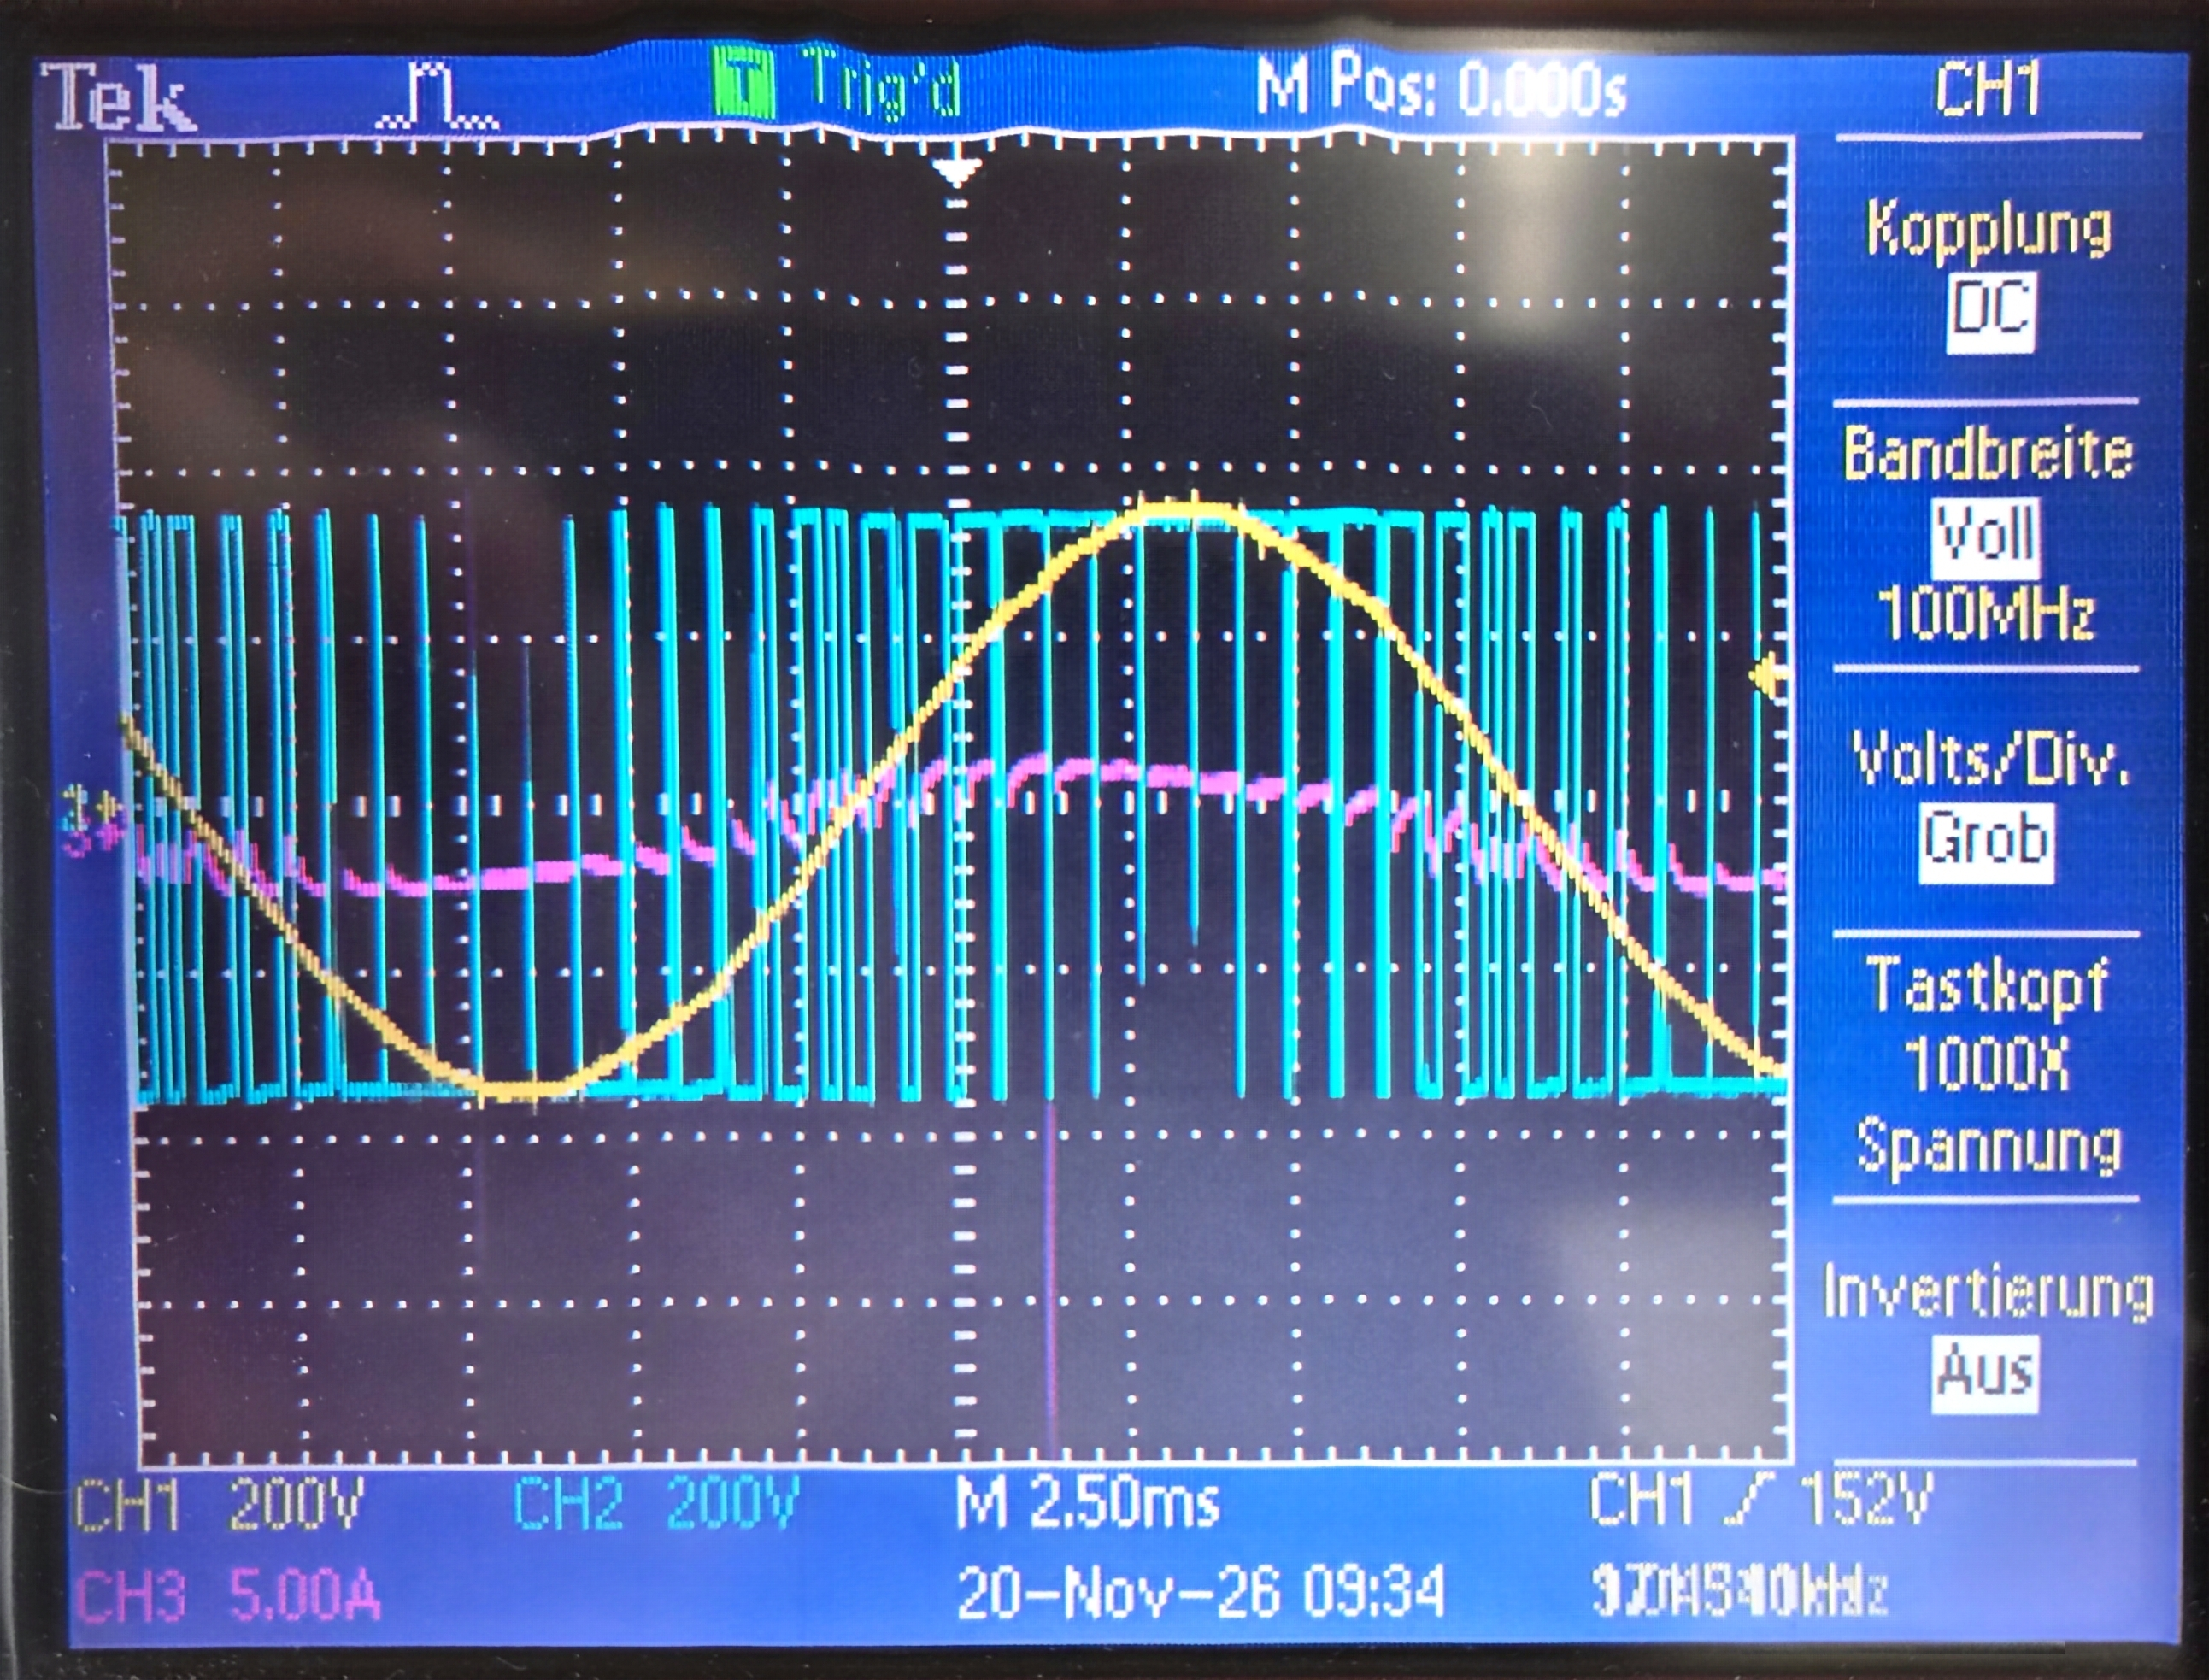
\includegraphics[width=\linewidth]{Scan_20261120_095904.jpg}
    \caption{Trägerverfahren fein, $\Udc=\SI{358}{\volt}$}
    \label{fig:621_fein}
  \end{subfigure}\hfill
  \begin{subfigure}[t]{0.48\linewidth}
    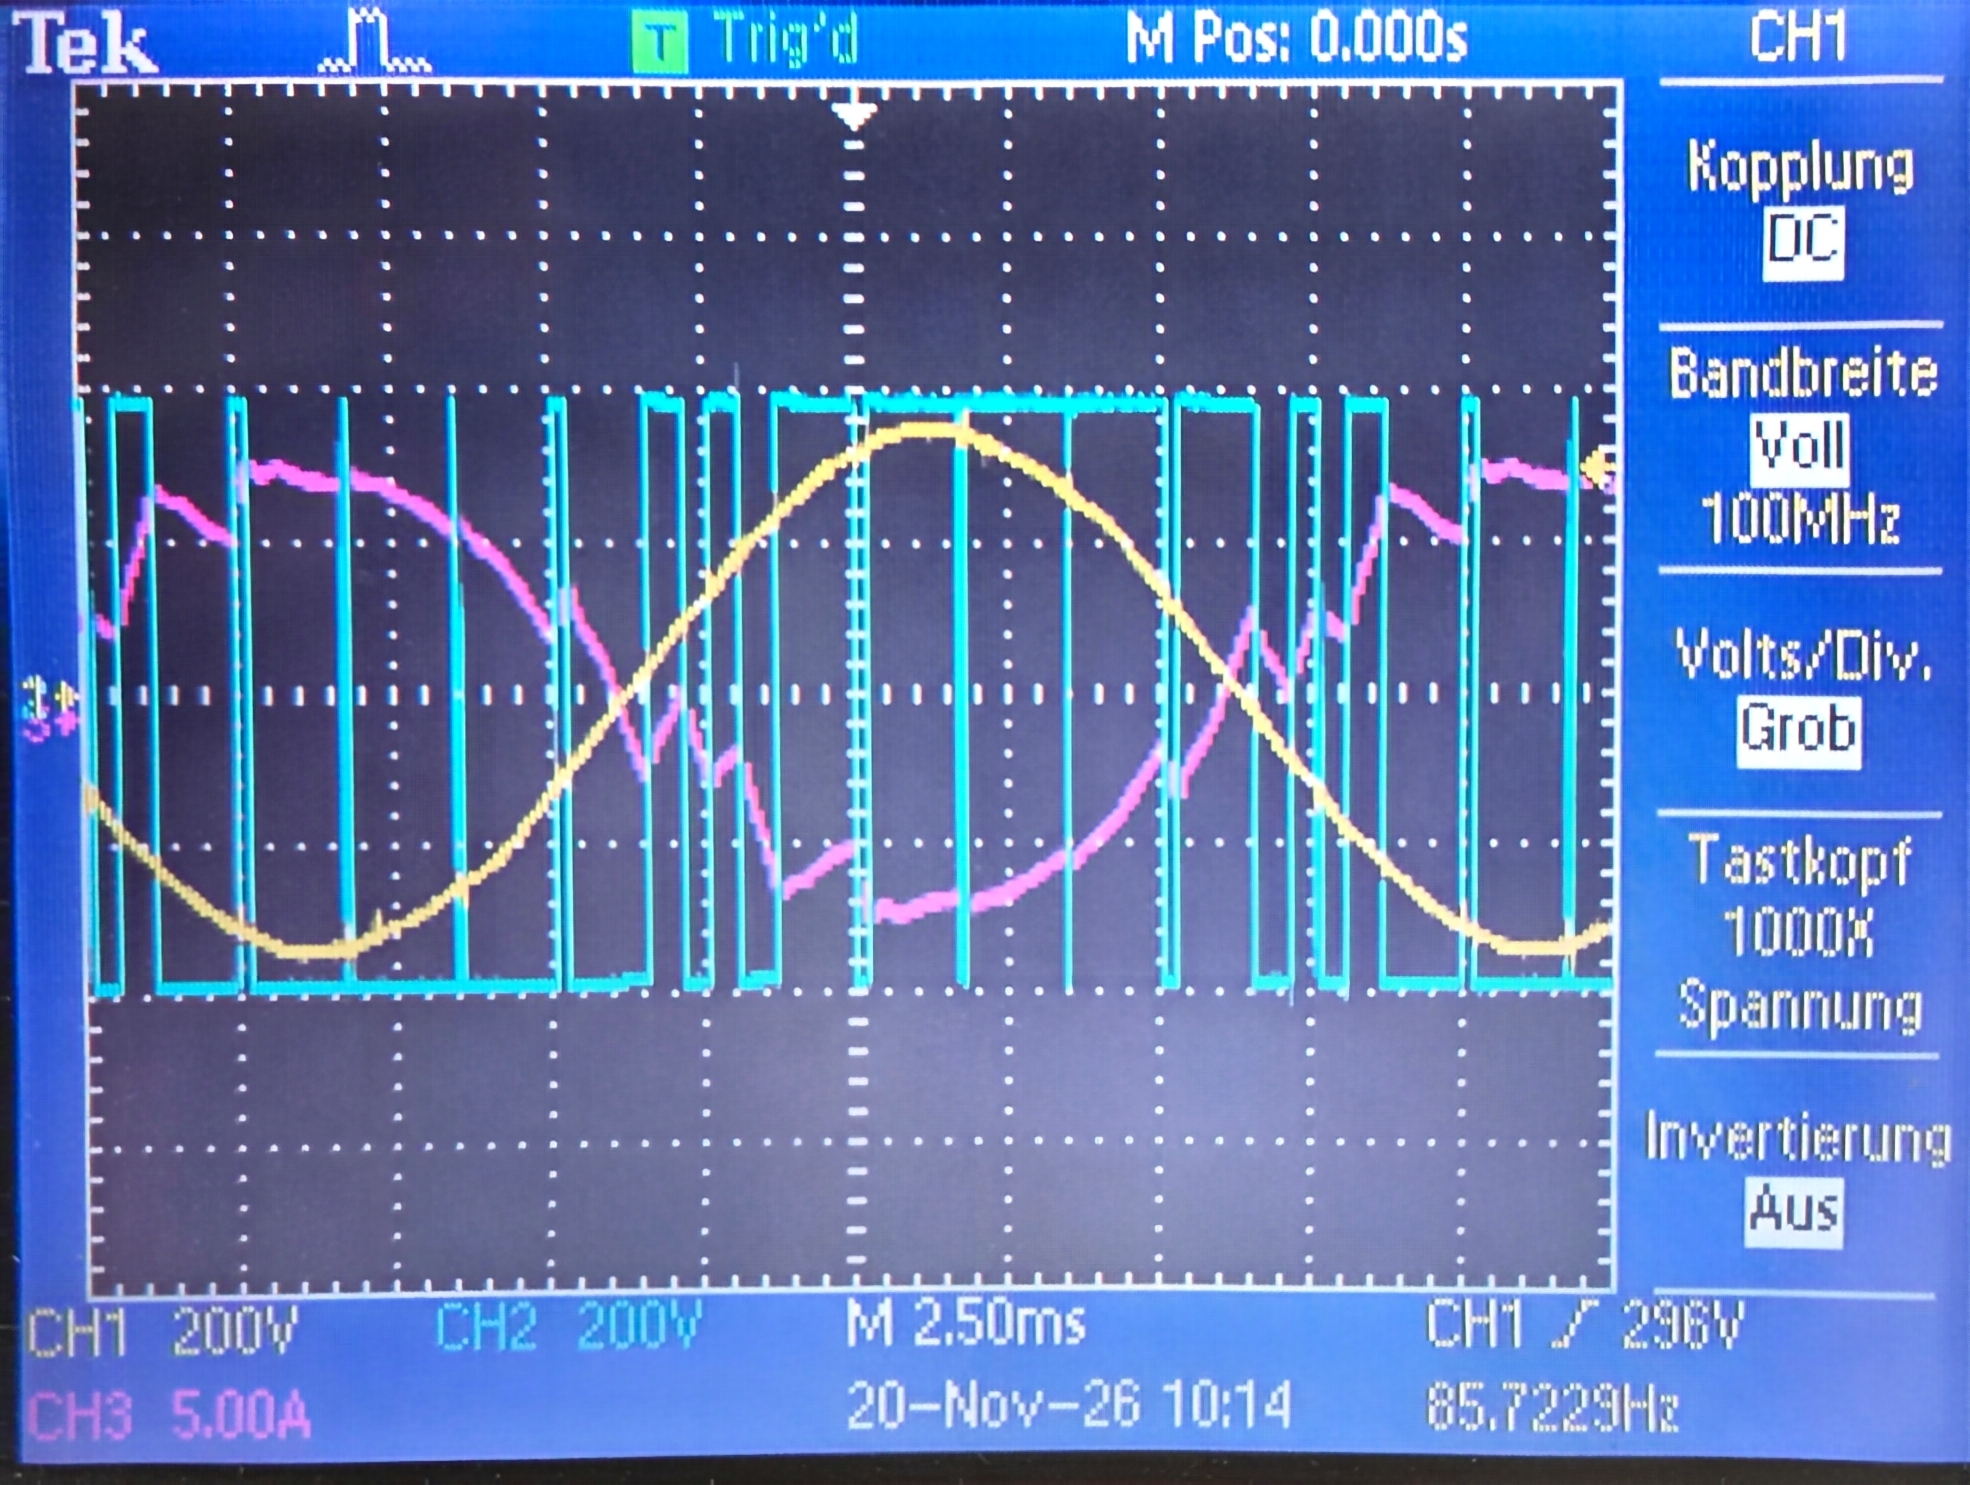
\includegraphics[width=\linewidth]{Scan_20261120_103938.jpg}
    \caption{Trägerverfahren grob, $\Udc=\SI{363}{\volt}$}
    \label{fig:621_grob}
  \end{subfigure}

  \medskip
  \begin{subfigure}[t]{0.48\linewidth}
    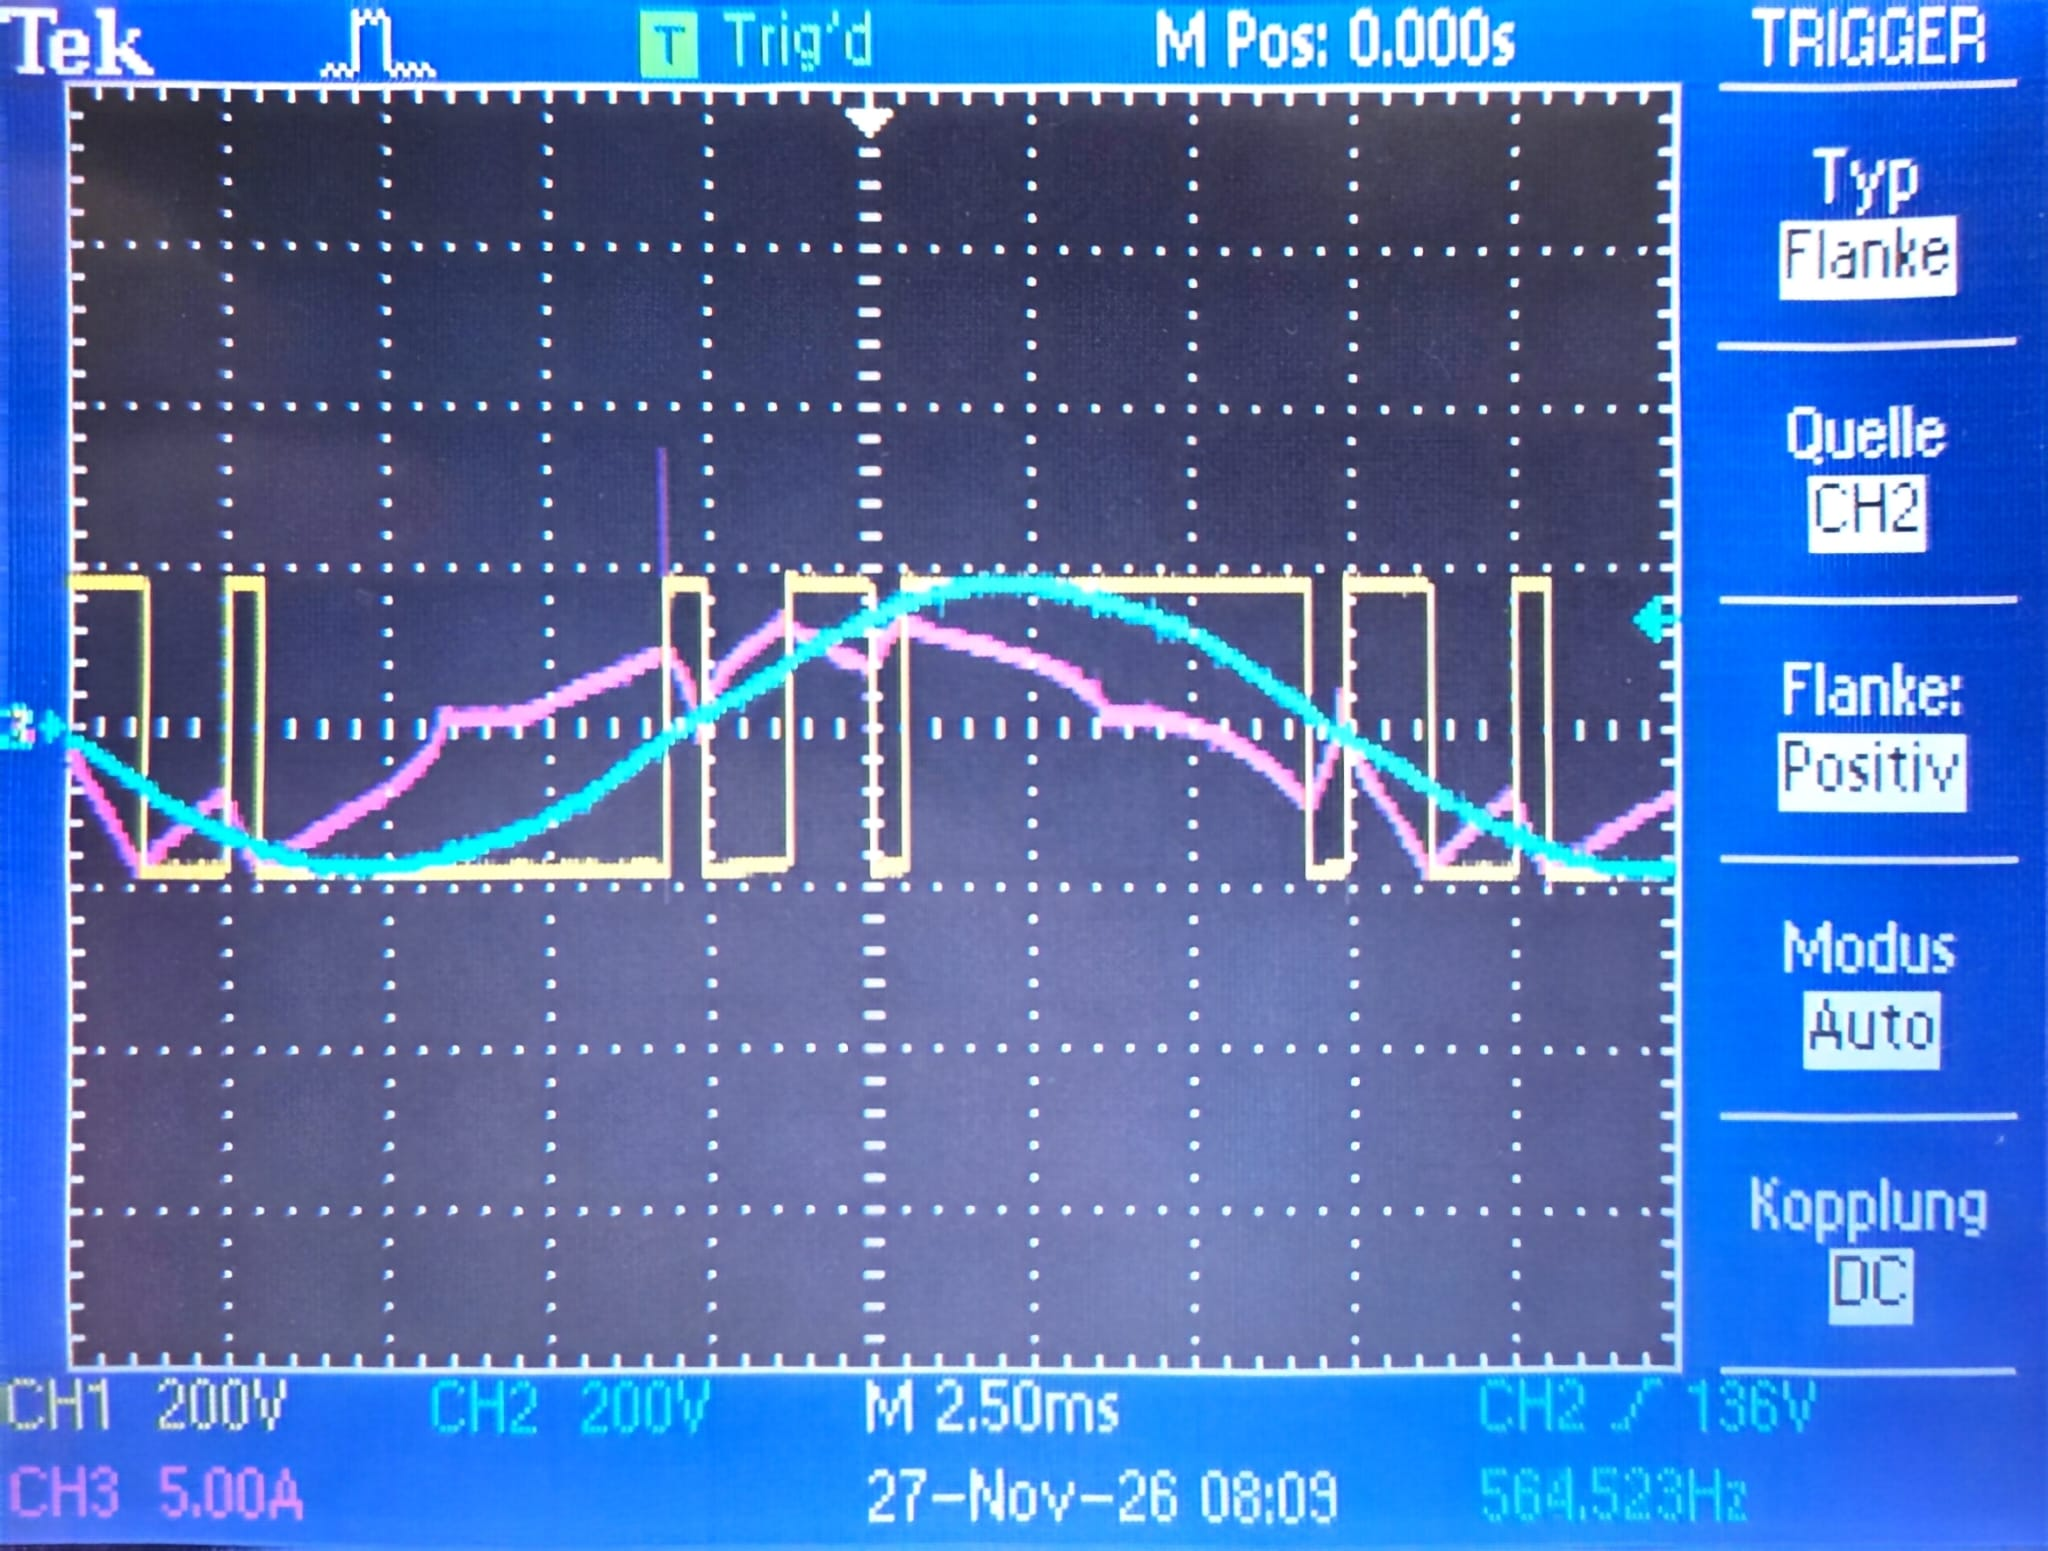
\includegraphics[width=\linewidth]{3_5_eliminiert.jpeg}
    \caption{«3.\ und 5.\ eliminiert», $\Udc=\SI{342}{\volt}$, $\Th=\SI{29.8}{\degree}$ (27.11.2026)}
    \label{fig:621_elim}
  \end{subfigure}\hfill
  \begin{subfigure}[t]{0.48\linewidth}
    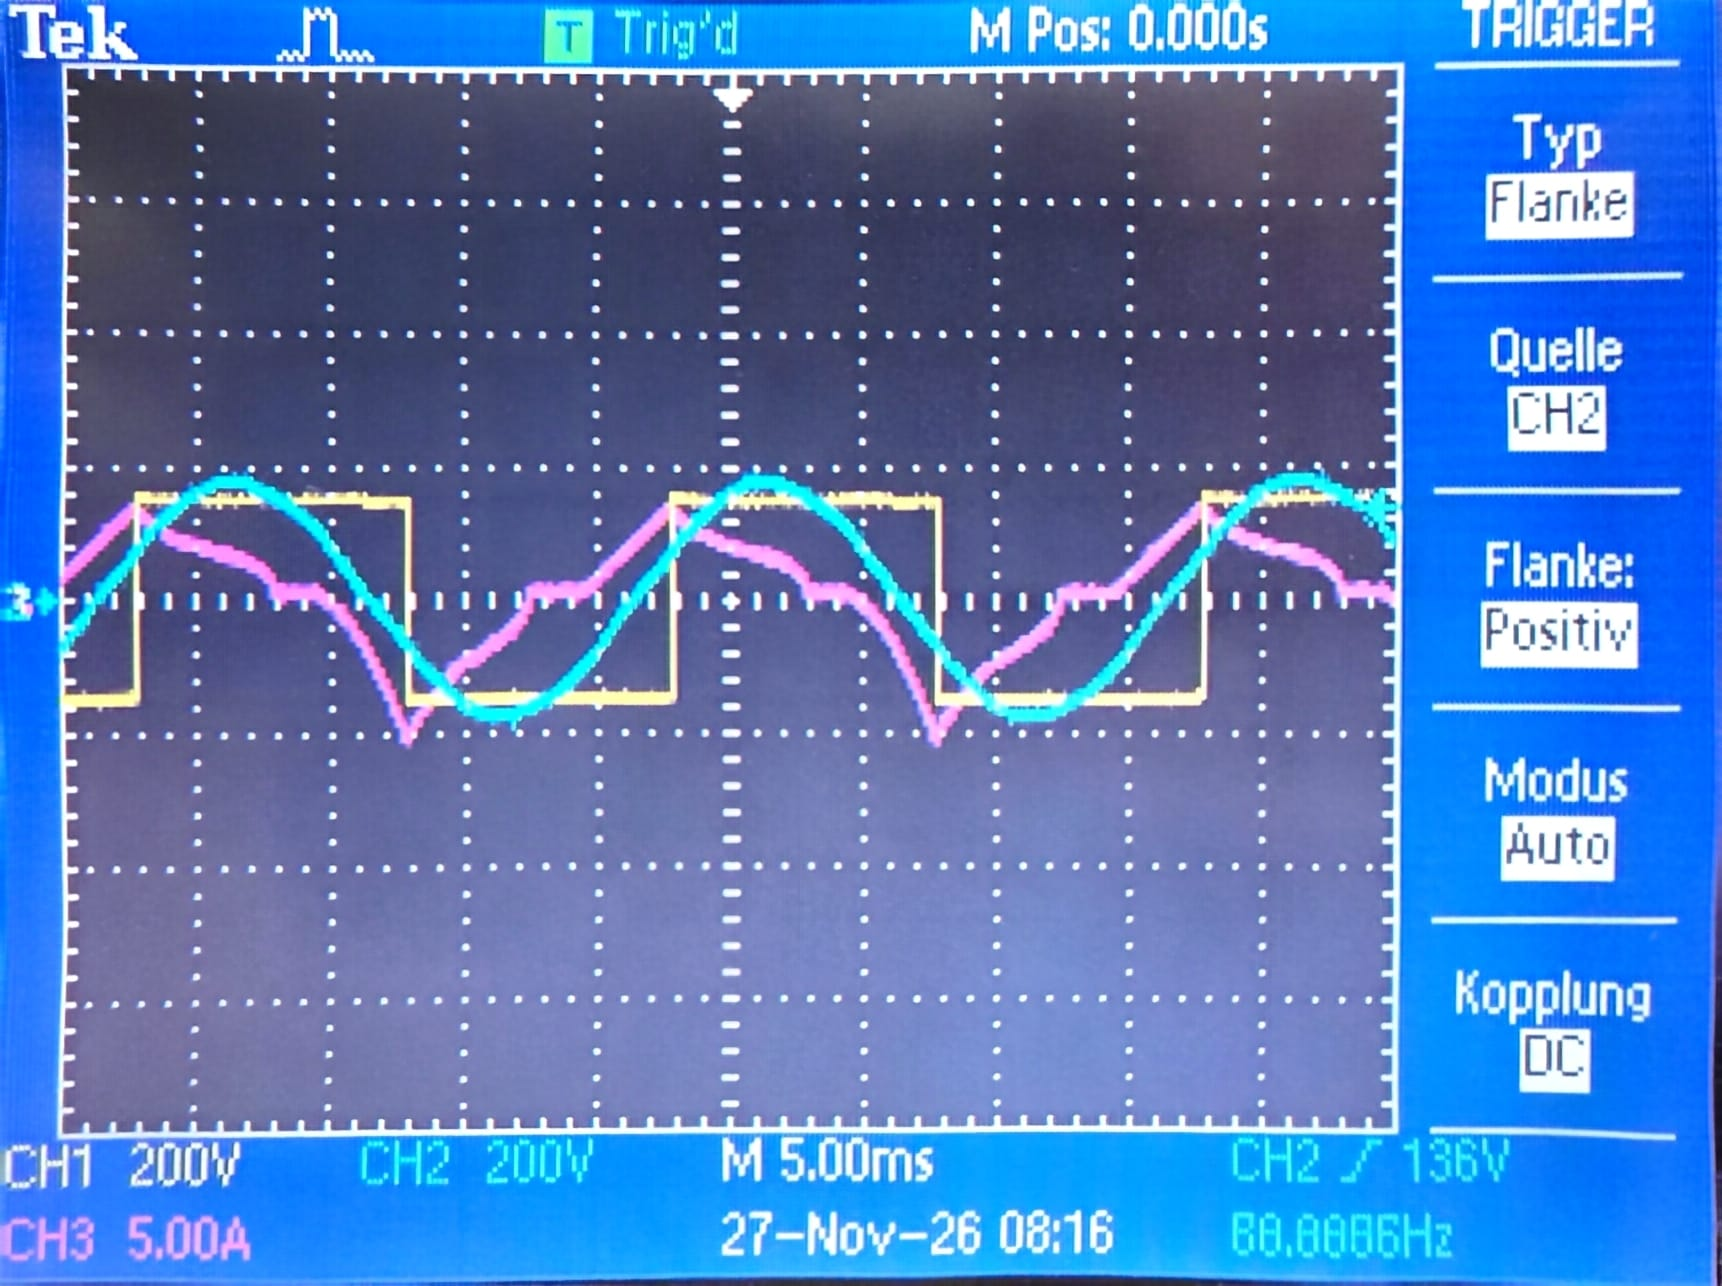
\includegraphics[width=\linewidth]{Grundferquenztaktung.jpeg}
    \caption{Grundfrequenztaktung (Referenz), $\Udc=\SI{284}{\volt}$, $\Th=\SI{28}{\degree}$ (27.11.2026, \SI{5}{\milli\second}/div)}
    \label{fig:621_rechteck}
  \end{subfigure}
  \caption{Oszillogramme am Lastpunkt $P\approx\SI{1.15}{\kilo\watt}$, $Q_1\approx0$. (a) und (b) vom 20.11.2026: Wechselrichterspannung (Cyan), Netzspannung (Gelb), Netzstrom (Magenta). (c) und (d) aus der Nachmessung vom 27.11.2026: Wechselrichterspannung (Gelb), Netzspannung (Cyan), Netzstrom (Magenta). Skalen: \SI{200}{\volt}/div, \SI{5}{\ampere}/div, \SI{2.5}{\milli\second}/div (Teilbild (d): \SI{5}{\milli\second}/div).}
  \label{fig:621}
\end{figure}

\paragraph{Beobachtungen.} Bei «3.\ und 5.\ eliminiert» ist $U_3=\SI{0.5}{\percent}$, die Elimination der 3.\ Oberschwingung ist damit bestätigt. Der gemessene Wert $U_5=\SI{30}{\percent}$ widerspricht der Erwartung (nahezu null); angesichts der stark schwankenden Anzeige (siehe unten) ist er vermutlich ein Ablesefehler. Dass $I_3=\SI{9}{\percent}$ trotz $U_3\approx0$ nicht verschwindet, könnte an einer Oberschwingung der Netzspannung liegen (Vermutung, $u_{\mathrm N}$ wurde nicht ausgewertet). Beim Trägerverfahren sind $U_3=\SI{20}{\percent}$ bzw.\ \SI{30}{\percent} unerwartet hoch, denn die Oberschwingungen sollten um die Schaltfrequenz liegen. Mögliche Ursachen sind Übermodulation (wenn die Grundschwingung am Rand des Aussteuerbereichs liegt), Ablesefehler oder ein anderer Prozentbezug (Vermutungen).

\paragraph{Messunsicherheit der Oberschwingungen.} Die Anzeige der Oberschwingungen am PM\,3000 schwankte bei den Pulsmustern stark; die abgelesenen Anteile streuten zwischen etwa \SI{2}{\percent} und \SI{50}{\percent}. Pro Grösse wurden deshalb mehrere Werte abgelesen und ungefähr gemittelt. Die Prozentwerte in Tabelle~\ref{tab:621_harm} sind daher nur grobe Richtwerte, und ein Vergleich der Muster auf wenige Prozentpunkte genau ist damit nicht möglich.

\paragraph{Stromformen.} Auf den Oszillogrammen ist der Unterschied der Muster gut zu sehen. Bei Grundfrequenztaktung (Abbildung~\ref{fig:621_rechteck}) ist der Strom stark verzerrt und hat bei jeder Schaltflanke eine Spitze. Beim Trägerverfahren «fein» besteht $\uWR$ aus einer sehr dichten Pulsfolge, und der Netzstrom verläuft nahezu glatt mit kleinem Schaltrippel. Bei «grob» gibt es deutlich weniger Pulse pro Netzperiode; der Strom ist sichtbar zackig und knickt bei jeder Schaltflanke. Beim Muster «3.\ und 5.\ eliminiert» (Abbildung~\ref{fig:621_elim}) ist $\uWR$ eine Rechteckspannung, in die an beiden Enden jeder Halbperiode zwei schmale Kerben geschnitten sind; die breite Mitte der Halbperiode bleibt erhalten. Der Strom ist dreieckförmig, mit einem Knick bei jeder Kerbe, und weniger spitz als bei Grundfrequenztaktung. Qualitativ ist der Strom bei «fein» damit am glattesten, was zur Theorie passt; die abgelesenen Prozentwerte zeigen das wegen ihrer Streuung nicht.

% ==========================================================================
\subsection{Aufgabe 6.2.2: Einstellen von \texorpdfstring{$P$ und $Q$}{P und Q} beim besten Muster}
\label{sec:messung622}

Die $P/Q$-Messungen für das beste Muster wurden aus Zeitgründen nicht durchgeführt.

\paragraph{Abschätzung von $\cos\varphi$ und $\lambda$.} Am Lastpunkt ist $Q_1\approx0$, also $\cos\varphi_1\approx1$. Der Leistungsfaktor $\lambda=P/S$ ist wegen der Oberschwingungsströme kleiner; bei sinusförmiger Netzspannung gilt $\lambda=\cos\varphi_1/\sqrt{1+\mathrm{THD}_I^2}$. Aus den abgelesenen $I_3$ und $I_5$ (Tabelle~\ref{tab:621_harm}) lässt sich $\mathrm{THD}_I$ nur nach unten abschätzen, weil die höheren Ordnungen fehlen; $\lambda$ ist damit eine obere Schranke (Tabelle~\ref{tab:622}). Wegen der Streuung der abgelesenen Werte sind das nur Grössenordnungen.

\begin{table}[htbp]
  \centering
  \caption{Abschätzung von $\mathrm{THD}_I$ und $\lambda$ aus $I_3$ und $I_5$ (berechnet, nicht gemessen; $\cos\varphi_1\approx1$).}
  \label{tab:622}
  \begin{tabular}{@{}lrr@{}}
    \toprule
    Pulsmuster & $\mathrm{THD}_I\gtrsim$ & $\lambda\lesssim$ \\
    \midrule
    3.\ und 5.\ eliminiert & \SI{11}{\percent} & 0.99 \\
    Trägerverfahren grob & \SI{24}{\percent} & 0.97 \\
    Trägerverfahren fein & \SI{36}{\percent} & 0.94 \\
    \bottomrule
  \end{tabular}
\end{table}

% ==========================================================================
\subsection{Aufgabe 6.3: Spannungsbelastung der Halbleiter}
\label{sec:messung63}

Erwartet wird für einen Halbleiter des Wechselrichters Folgendes (Skizze in Abbildung~\ref{fig:halbleiter_skizze}): Die Spannung über dem Schalter ist null, solange er leitet, und gleich der vollen Zwischenkreisspannung $\Udc$, solange er sperrt. Beim Schalten können Überschwinger auftreten. Der Strom entspricht im Leitintervall dem Netzstrom $\iN$; je nach Stromrichtung führt ihn der IGBT oder die antiparallele Diode.

\begin{figure}[htbp]
  \centering
  \begin{tikzpicture}
    \begin{axis}[rep,height=3.6cm,xlabel={},ylabel={$u_{\mathrm T}$},
        xmin=0,xmax=360,xtick={0,90,...,360},ymin=-0.2,ymax=1.3,ytick={0,1},yticklabels={0,$\Udc$}]
      \addplot[thick,domain=0:360,samples=721]{ifthenelse(x<180,0,1)};
    \end{axis}
  \end{tikzpicture}

  \begin{tikzpicture}
    \begin{axis}[rep,height=3.6cm,xlabel={$\omega t$ in \si{\degree}},ylabel={$i_{\mathrm T}$ in A},
        xmin=0,xmax=360,xtick={0,90,...,360},ymin=-5,ymax=5]
      \addplot[thick,domain=0:360,samples=721]{ifthenelse(x<180,(255.46*(x*pi/180-pi/2)+325.27*cos(x))/21.99,0)};
    \end{axis}
  \end{tikzpicture}
  \caption{Skizze (Erwartung) von Spannung $u_{\mathrm T}$ und Strom $i_{\mathrm T}$ des oberen Schalters für den Fall aus Abschnitt~\ref{sec:vorbereitung}: Der Strom fliesst im Leitintervall; seine positiven Anteile laufen über den IGBT, die negativen über die Diode (je nach Stromrichtung).}
  \label{fig:halbleiter_skizze}
\end{figure}

\begin{figure}[htbp]
  \centering
  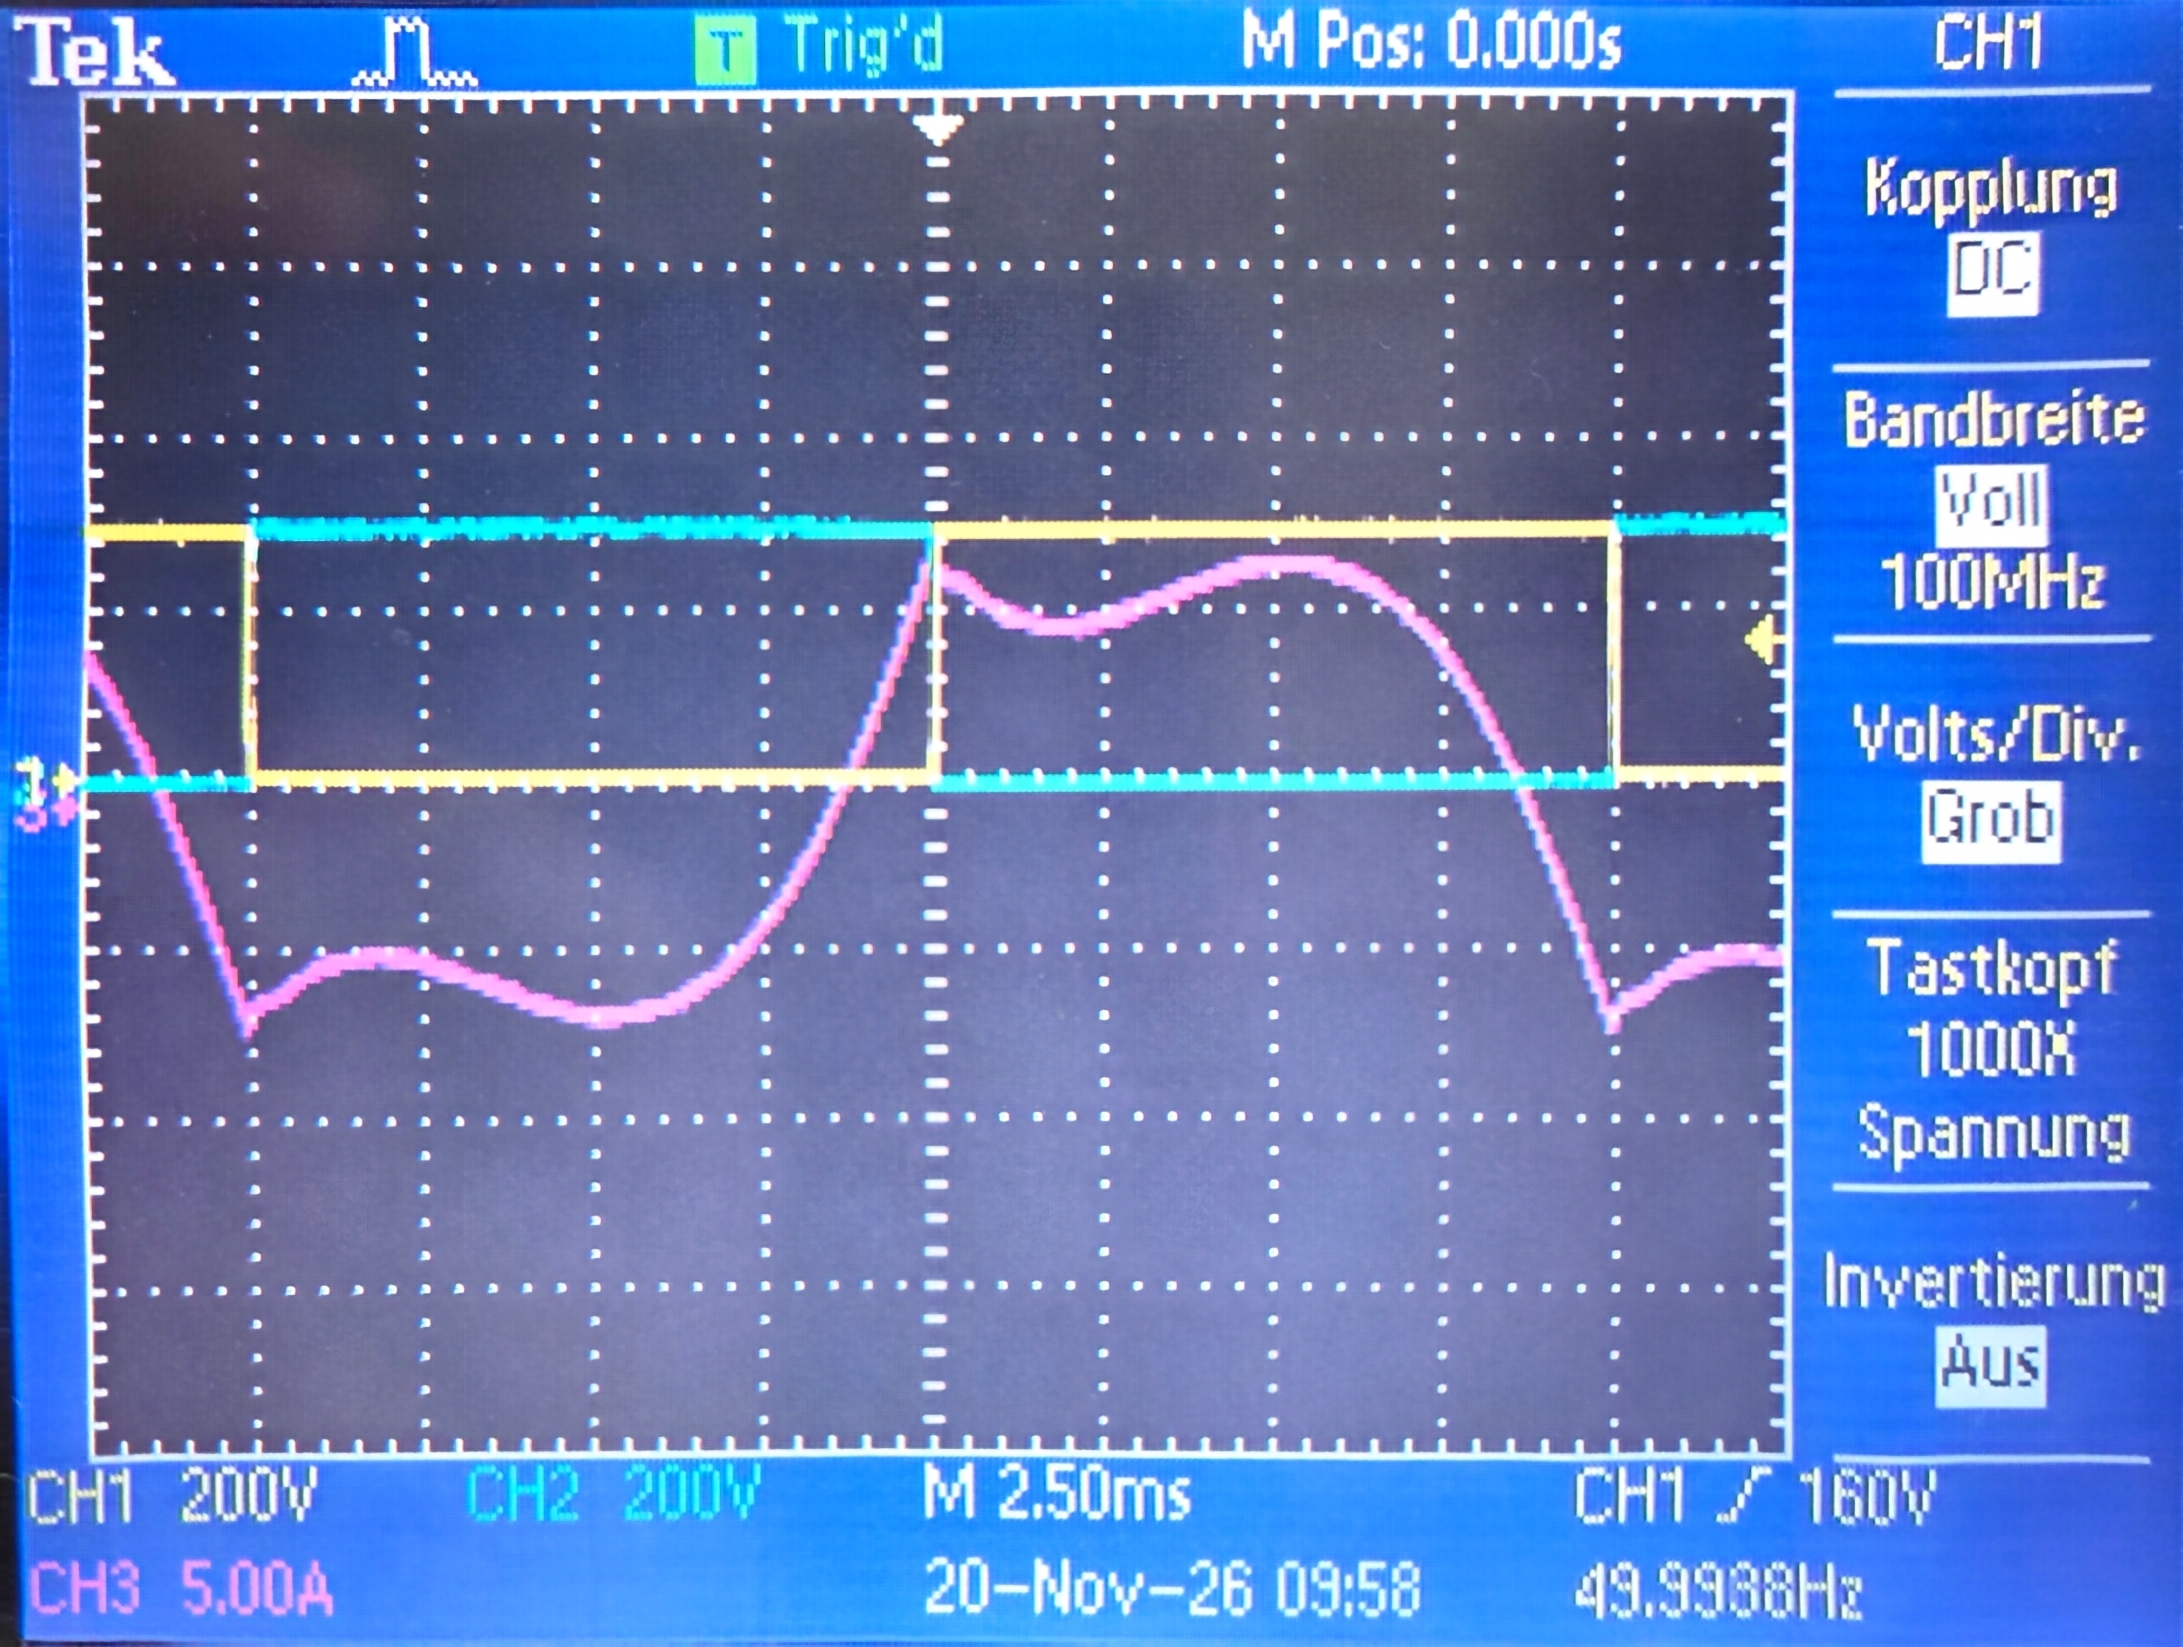
\includegraphics[width=0.62\linewidth]{Scan_20261120_102240.jpg}
  \caption{Aufgabe 6.3, Oszillogramm (20.11.2026, 09:58). Skalen: \SI{200}{\volt}/div (CH1, CH2), \SI{5}{\ampere}/div (CH3), \SI{2.5}{\milli\second}/div.}
  \label{fig:halbleiter_mess}
\end{figure}

Gemessen wurde bei Grundfrequenztaktung. Das Oszillogramm zeigt zwei zueinander komplementäre Rechteckspannungen (Gelb, Cyan) mit einem Hub von rund \SI{290}{\volt}, was der Zwischenkreisspannung entspricht. Es sind die Spannungen über zwei Halbleitern, und zwar Cyan über dem Schalter, der die positive Halbwelle von $\uWR$ schaltet, und Gelb über dem Schalter der negativen Halbwelle. Magenta ist der Netzstrom $\iN$. Die Flanken sind sauber, bei \SI{200}{\volt}/div sind keine Überschwinger zu erkennen. Der Netzstrom ändert bei jeder Schaltflanke seine Steigung, wie es $L\,\mathrm{d}i/\mathrm{d}t=\uWR-\uN$ verlangt; er fliesst durch den Halbleiter, solange dieser leitet.

% ==========================================================================
\subsection{Aufgabe 6.4: Drehzahl der Asynchronmaschine}
\label{sec:messung64}

Die Drehzahl wurde mit dem optischen Drehzahlmesser gemessen. Tabelle~\ref{tab:drehzahl} stellt die gemessenen Werte den Angaben auf dem Typenschild gegenüber. Im Leerlauf wurden \SI{1500}{\per\minute} gemessen; das entspricht der Synchrondrehzahl und dem Wert auf dem Typenschild.

\begin{table}[htbp]
  \centering
  \caption{Drehzahl der ASM: gemessene Werte und Angaben auf dem Typenschild.}
  \label{tab:drehzahl}
  \begin{tabular}{@{}llr@{}}
    \toprule
    Zustand & Quelle & $n$ in \si{\per\minute} \\
    \midrule
    Leerlauf & gemessen & 1500 \\
    Nennlast & Typenschild & 1430 \\
    Generatorbetrieb, $P\approx\SI{1.1}{\kilo\watt}$ & gemessen & 1505 \\
    Motorbetrieb, $P\approx\SI{-1.1}{\kilo\watt}$ ($\Th=\SI{-15}{\degree}$, $\Udc=\SI{288}{\volt}$) & gemessen & 1488.8 \\
    \bottomrule
  \end{tabular}
\end{table}

Der Betriebszustand der ASM folgt aus der Leistungsrichtung (Abschnitt~\ref{sec:vorzeichen}). Bei $P>0$ arbeitet der Wechselrichter als Gleichrichter und treibt die GM als Motor an; die ASM wird dann übersynchron angetrieben und arbeitet als Generator, hier bei \SI{1505}{\per\minute}. Bei $P<0$ speist der Wechselrichter in das Netz~2 zurück, die GM ist Generator und die ASM Motor; sie läuft untersynchron, hier bei \SI{1488.8}{\per\minute}. Die lastpunktbezogenen Messungen der übrigen Aufgaben fanden im Generatorbetrieb statt; der Motorbetrieb wurde nur für diese Drehzahlmessung durch Ändern des Winkels eingestellt.

Gemessen liegt die Drehzahl damit zwischen etwa \SI{1489}{\per\minute} und \SI{1505}{\per\minute}, also nur rund $\pm\SI{0.5}{\percent}$ um die Synchrondrehzahl von \SI{1500}{\per\minute}; die ASM hält die Drehzahl wie vorausgesetzt praktisch konstant. Daraus ergibt sich im Motorbetrieb ein Schlupf von $s=(1500-1488.8)/1500\approx\SI{0.75}{\percent}$ und im Generatorbetrieb von $s\approx\SI{-0.33}{\percent}$ (berechnet). Der Typenschildwert von \SI{1430}{\per\minute} bei Nennlast entspricht einem Schlupf von rund \SI{4.7}{\percent}; er wurde nicht gemessen, da die Nennlast nicht gefahren wurde. Die Synchrondrehzahl von \SI{1500}{\per\minute} bei \SI{50}{\hertz} entspricht der Polpaarzahl $p=2$; diese wurde aus der Drehzahl abgeleitet und nicht auf dem Typenschild geprüft.

% !TEX root = ../main.tex
\section{Diskussion}
\label{sec:diskussion}

\paragraph{Übereinstimmung mit der Theorie.} Bei Grundfrequenztaktung stimmen die gemessenen Spannungs- und Stromoberschwingungen sehr gut mit \eqref{eq:rechteck} und \eqref{eq:In} überein (Tabelle~\ref{tab:611}). Auch die Abhängigkeit $P\propto\sin\Th$ und das Minimum von $Q$ nahe $U_{\mathrm{WR1}}\approx\UN$ werden bestätigt. Der Grundschwingungsstrom liess sich nicht auf null bringen; $I_1=\SI{0.827}{\ampere}$ entspricht rund \SI{18}{\volt} Differenz zwischen $U_{\mathrm{WR1}}$ und $\UN$ und ist im Vergleich zu den Oberschwingungsströmen klein.

\paragraph{Winkel-Offset.} Die Wirkleistung wird nicht bei $\Th=0$, sondern bei $\Th\approx\SI{4.7}{\degree}$ null. Mögliche Ursachen sind die Synchronisation, Verluste in Wechselrichter, Drossel und Transformator oder Messtoleranzen. Eine Überprüfung (z.\,B.\ Messung der Phasenlage von $\uN$ und $\uWR$ am Oszilloskop) wurde nicht durchgeführt.

\paragraph{Blindleistung.} Das am PM\,3000 abgelesene $Q$ enthält die Verzerrungsblindleistung und erreicht deshalb nie null. Sein Minimum ($\Udc\approx250$ bis \SI{275}{\volt}) liegt nahe der Stelle, an der $U_{\mathrm{WR1}}=\UN$ ist; die Aufgabe verlangt jedoch $Q_1$. Da $I_1$ und $P_1$ nicht notiert wurden, konnte $Q_1$ nicht angegeben werden.

\paragraph{Lastpunkt.} Der in der Anleitung genannte Lastpunkt $P=\SI{1.5}{\kilo\watt}$, $Q_1=0$ wurde nicht erreicht; der Vergleich der Pulsmuster fand bei \SI{1.15}{\kilo\watt} statt. Weil alle Muster am selben Lastpunkt gemessen wurden, bleibt der Vergleich untereinander gültig.

\paragraph{Ausnutzung der Zwischenkreisspannung.} Für denselben Lastpunkt braucht das Trägerverfahren mit $\Udc\approx\SI{360}{\volt}$ deutlich mehr Zwischenkreisspannung als «3.\ und 5.\ eliminiert» mit \SI{282}{\volt}. Die Trägerverfahren nutzen die Gleichspannung also schlechter aus; das ist ein Nachteil, den die Theorie mit den kleineren Strom-Oberschwingungen bei hoher Schaltfrequenz aufwiegt.

\paragraph{Bestes Muster.} Nach den eigenen Messwerten hat «3.\ und 5.\ eliminiert» die kleinsten Stromoberschwingungen ($I_3=\SI{9}{\percent}$, $I_5=\SI{7}{\percent}$). Die Theorie würde bei hoher Schaltfrequenz («Trägerverfahren fein») Vorteile erwarten, weil die Oberschwingungen dann bei hohen Ordnungen liegen und von der Induktivität stark gedämpft werden. Die Messwerte zeigen das nicht: Für «fein» sind $U_3=\SI{20}{\percent}$ und $I_5=\SI{30}{\percent}$ unerwartet hoch. Mögliche Ursachen sind Übermodulation (Grundschwingung am Rand des Aussteuerbereichs), Ablese- oder Notierfehler oder ein unklarer Prozentbezug (Vermutungen). Ein eindeutiger Vergleich bräuchte $\mathrm{THD}_I$ aller Muster.
\paragraph{Unstimmigkeiten in den Messdaten.} Folgende Punkte bleiben offen und sind im Bericht als \texttt{todo}-Boxen markiert:
\begin{itemize}
  \item $Q$ bei $\Udc=\SI{350}{\volt}$ in Tabelle~\ref{tab:udc} fehlt.
  \item $P_1$, $Q_1$ und $I_3$ in Aufgabe~6.1.2 wurden nicht aufgenommen.
  \item «3.\ und 5.\ eliminiert»: $U_5=\SI{30}{\percent}$ und $I_1=\SI{1.2}{\ampere}$ sind unplausibel.
  \item Trägerverfahren: $U_3=\SI{20}{\percent}$ bis \SI{30}{\percent} ist für ein Trägerverfahren unerwartet hoch.
  \item Aufgabe~6.2.2: $P/Q$-Tabelle, $\cos\varphi$ und $\lambda$ fehlen.
  \item Aufgabe~6.3: Spurzuordnung im Oszillogramm fehlt.
  \item Aufgabe~6.4: Zuordnung der Einstellung «$-15^\circ$, \SI{288}{\volt}» zu einem Lastzustand ist unklar.
\end{itemize}

% !TEX root = ../main.tex
\section{Fazit}
\label{sec:fazit}

Die Fragen der Versuchsanleitung lassen sich anhand der Messungen wie folgt beantworten:

\begin{itemize}
  \item \emph{Wie beeinflusst man $P$ und $Q$?} Die Wirkleistung wird über den Winkel $\Th$ eingestellt ($P\propto\sin\Th$), die Blindleistung über die Amplitude $U_{\mathrm{WR1}}$, am Versuch also über $\Udc$ (Abschnitte~\ref{sec:vorbereitung} und \ref{sec:messung612}).
  \item \emph{Welche Harmonischen treten bei Grundfrequenztaktung auf?} Es treten nur ungerade Ordnungen auf. $U_n$ fällt mit $1/n$, $I_n$ mit $1/n^2$ ab; die Messung bestätigt die Theorie (Tabelle~\ref{tab:611}).
  \item \emph{Einfluss von $\Th$ und $\Udc$ auf die Harmonischen?} Theoretisch ist $I_n$ proportional zu $\Udc$ und unabhängig von $\Th$; dies wurde nicht gemessen.
  \item \emph{Stromform und Oberschwingungen je Pulsmuster?} Bei \SI{1.15}{\kilo\watt} und $Q_1\approx0$ hatte «3.\ und 5.\ eliminiert» die kleinsten Stromoberschwingungen ($I_3=\SI{9}{\percent}$, $I_5=\SI{7}{\percent}$); die Trägerverfahren brauchten rund \SI{360}{\volt} statt \SI{282}{\volt} Zwischenkreisspannung (Abschnitt~\ref{sec:messung621}). Die Theorie erwartet für das feine Trägerverfahren die kleineren Oberschwingungen; dieser Widerspruch bleibt wegen der stark schwankenden Anzeige als Beobachtung stehen.
  \item \emph{Funktioniert die $P$/$Q$-Einstellung bei den anderen Pulsmustern gleich?} Der gleiche Winkel genügte für alle Muster am Lastpunkt; $\Udc$ muss höher gewählt werden. Eine vollständige Messreihe fehlt (Abschnitt~\ref{sec:messung622}).
  \item \emph{Optimaler $\cos\varphi$ und $\lambda$?} Nicht gemessen.
  \item \emph{Verläufe an den Halbleitern?} Erwartung als Skizze, Messung als Oszillogramm: komplementäre Rechteckspannungen mit dem Hub $\Udc$, Strom mit Steigungswechsel bei jeder Flanke; die Spurzuordnung beruht auf einer Vermutung (Abschnitt~\ref{sec:messung63}).
  \item \emph{Drehzahlbereich der ASM?} Gemessen etwa \SI{1489}{\per\minute} (Motorbetrieb, \SI{1.15}{\kilo\watt}) bis \SI{1505}{\per\minute} (Generatorbetrieb, \SI{1.15}{\kilo\watt}); laut Typenschild \SI{1500}{\per\minute} im Leerlauf und \SI{1430}{\per\minute} bei Nennlast (Abschnitt~\ref{sec:messung64}).
\end{itemize}


% ---------------------------------------------------------------- KI-Deklaration
\section*{Deklaration zur Verwendung von KI}
\addcontentsline{toc}{section}{Deklaration zur Verwendung von KI}

Bei der Erstellung dieses Berichts wurde das KI-Sprachmodell Claude (Anthropic) eingesetzt, und zwar wie folgt:
\begin{itemize}
  \item \emph{Während der Messungen:} für Verständnisfragen zum Versuch, zur Bedienung des Aufbaus und zur Interpretation der Messgrössen.
  \item \emph{Beim Schreiben:} für die Strukturierung des Berichts, für das Formulieren von Textabschnitten und für LaTeX-Code (Tabellen, Diagramme, Zeigerdiagramme).
  \item \emph{Bei der Korrektur:} für die Prüfung auf inhaltliche Widersprüche, Rechenfehler, Plausibilität der Messwerte, Sprache und Formales.
\end{itemize}
Alle Messungen haben wir selbst durchgeführt und die Messwerte selbst erhoben. Die Vorschläge der KI haben wir geprüft, mit unseren Messdaten und den Unterlagen verglichen und bei Bedarf angepasst. Für den Inhalt des Berichts sind die Autoren verantwortlich.

% ---------------------------------------------------------------- Quellen
\begin{thebibliography}{9}
  \bibitem{anleitung} A.~Omlin: \emph{Versuchsanleitung LEAS -- Wechselrichter einphasig}. Hochschule Luzern -- Technik \& Architektur, Stand 08.11.2024.
  \bibitem{skript} A.~Omlin: \emph{Skript ET+A}, Kapitel «Wechselrichter». Hochschule Luzern -- Technik \& Architektur, 2026.
\end{thebibliography}

\end{document}
